%% ============================================================================
%% Sensitivity of 2D flood models to Manning roughness uncertainty:
%% a Monte Carlo comparison of SFINCS and HEC-RAS in the Besaya River
%% ============================================================================
\documentclass[a4paper,fleqn]{cas-sc}

\usepackage{amsmath,amssymb}
\usepackage{booktabs}
\usepackage{array}
\usepackage{multirow}
\usepackage{siunitx}
\usepackage[authoryear,longnamesfirst]{natbib}
\usepackage{lineno}
\usepackage{setspace}
\usepackage{pdflscape}

% Compatibility for CAS 2.4 with newer LaTeX3 kernels.
\ExplSyntaxOn
\cs_if_exist:NF \vbox_unpack_clear:N
  { \cs_new_eq:NN \vbox_unpack_clear:N \vbox_unpack_drop:N }
% Patch: suppress empty "ORCID(s):" label when orcid is set via \ead[orcid]{}.
\RenewDocumentCommand \printorcid { }
{
  \seq_if_empty:NF \g_stm_orcid_seq
  {
    \group_begin:
      \tex_let:D \thefootnote \relax \footnotetext
      {
        \raggedright
        \textsc{orcid}(s):\c_space_token
        \seq_use:Nn \g_stm_orcid_seq { ;~ }
      }
    \group_end:
  }
}
\ExplSyntaxOff

\linenumbers
\doublespacing

% convenience macros
\newcommand{\nman}{$n$}
\newcommand{\CV}{\text{CV}}
\newcommand{\sfincs}{\textsc{SFINCS}}
\newcommand{\hecras}{\textsc{HEC-RAS}}

%% ===========================================================================
\begin{document}
\let\WriteBookmarks\relax
\def\floatpagepagefraction{1}
\def\textpagefraction{.001}

\shorttitle{Roughness uncertainty and model-structure effects}
\shortauthors{Navas et~al.}

\title[mode=title]{From roughness uncertainty to model-structure effects in 2D flood inundation models: a Monte Carlo comparison of SFINCS and HEC-RAS}

\author[1]{Salvador Navas}
\cormark[1]
\ead{salvador.navas@hidralab.com}
\ead[orcid]{0000-0001-7439-1743}
\credit{Conceptualization, Methodology, Software, Data curation, Formal analysis, Visualization, Writing -- original draft, Writing -- review \& editing}

\affiliation[1]{organization={HidraLab},
                addressline={Avda. Camilo Jos\'e Cela s/n},
                city={Ciudad Real},
                postcode={13005},
                country={Spain}}

\author[2]{\'Alvaro Gal\'an}
\credit{Conceptualization, Writing -- review \& editing}

\affiliation[2]{organization={Escuela T\'ecnica Superior de Ingenier\'ia de Caminos, Canales y Puertos, Universidad de Castilla-La Mancha},
                addressline={Avda. Camilo Jos\'e Cela s/n},
                city={Ciudad Real},
                postcode={13005},
                country={Spain}}

\author[3]{Manuel del Jesus}
\credit{Resources, Supervision, Funding acquisition, Writing -- review \& editing}

\affiliation[3]{organization={Escuela T\'ecnica Superior de Ingenieros de Caminos, Canales y Puertos, Universidad de Cantabria},
                addressline={Avda. de los Castros s/n},
                city={Santander},
                postcode={39005},
                country={Spain}}

\cortext[1]{Corresponding author}

%% ---------------------------------------------------------------------------
\begin{abstract}
Manning roughness uncertainty in 2D flood models is usually assessed within a
single model structure. We compare SFINCS and HEC-RAS --- configurations that
differ in governing-equation approximation, mesh design and numerical
implementation --- using a paired Monte Carlo ensemble of 995 valid roughness
realisations for a $T=500$-year design flood in the Besaya River floodplain,
northern Spain. Spatially averaged Manning values explain less than 2\% of
domain-scale flood-output variance in either model, yet the same inputs produce
contrasting uncertainty structures. HEC-RAS shows larger ensemble variability
than SFINCS and a bimodal flooded-area distribution, whereas SFINCS remains
narrow and unimodal. Spatial inundation-frequency maps link the HEC-RAS regimes
to a 60.1~m topographic saddle controlling access to a 7.4~ha secondary
floodplain compartment. The bimodality persists under alternative metrics and
correlated-roughness robustness checks, indicating that the complete modelling
configuration, not only the governing equations, can alter the shape of
probabilistic flood-hazard distributions near threshold-controlled topographic
features. This finding is based on a single site and a single return period;
whether threshold-controlled bimodal responses are a general feature of
full-momentum models in floodplains with saddle-controlled secondary compartments
remains an open question requiring testing across additional sites and event
magnitudes.
\end{abstract}

\begin{highlights}
\item Paired roughness ensemble compares SFINCS and HEC-RAS flood responses.
\item Mean Manning explains less than 2\% of output variance in both models.
\item HEC-RAS yields a bimodal area response; SFINCS remains unimodal.
\item A 60.1 m saddle controls access to a secondary floodplain compartment.
\item Model configuration --- not governing equations alone --- determines the shape of the uncertainty distribution.
\end{highlights}

\begin{keywords}
Manning roughness \sep Monte Carlo simulation \sep 2D flood modelling \sep
SFINCS \sep HEC-RAS \sep model-structure uncertainty \sep flood hazard
\end{keywords}

\maketitle

%% ===========================================================================
\section{Introduction}
\label{sec:intro}
Flood inundation models are now routinely used to support flood hazard mapping, emergency planning, infrastructure design and risk assessment. Their role is not only to reproduce water levels at a few control points, but to translate hydrological forcing into spatially distributed estimates of water depth, velocity and inundation extent. This is particularly important in urban and semi-urban floodplains, where small differences in routing can determine whether roads, industrial areas or secondary floodplain compartments become connected to the main flow. Recent reviews have shown that two-dimensional hydrodynamic models have become central to this task, while also stressing that uncertainty remains a persistent limitation in their operational use \citep{teng2017}.

Uncertainty in flood inundation modelling arises from several sources. Topographic data, boundary conditions, numerical discretisation, model formulation and hydraulic parameters can all affect predicted flood extent and depth \citep{pappenberger2005,apel2008,merwade2008,teng2017}. Among the hydraulic parameters, Manning's roughness coefficient is one of the most commonly adjusted and one of the most difficult to specify objectively. In practical studies, roughness values are usually assigned by land-use class using published tables, previous experience and visual interpretation of aerial imagery or field observations \citep{chow1959,barnes1967,fhwa1984,brater1996}. These sources provide useful reference ranges, but they do not remove the ambiguity associated with vegetation state, local channel conditions, urban surfaces, flow depth or seasonal variability.

The effect of Manning's coefficient on 2D flood simulations is therefore not a simple matter of choosing a single representative value. Roughness enters the momentum balance through a non-linear friction term, so changes in \nman{} interact with water depth, velocity and local topography. Monte Carlo methods provide a practical framework for propagating this uncertainty through hydraulic models: roughness values are sampled from plausible distributions, the model is run repeatedly, and the resulting ensemble is used to characterise the variability of flood outputs. This approach is consistent with the broader use of sensitivity and uncertainty analysis in environmental modelling, where the objective is to understand how uncertain inputs affect model outputs and, ultimately, the robustness of model-based decisions \citep{saltelli2010,pianosi2016}.

Previous flood-inundation studies have shown that Manning uncertainty can affect simulated water levels, floodplain margins and local hazard metrics, although its influence on domain-averaged quantities is often weaker than might be expected \citep{aronica2002,hall2005,pappenberger2005,fewtrell2011,savage2016,pinos2023,ulate2024}. This difference between local and aggregated responses is important. A small change in roughness may have little effect on mean flooded area over an entire domain, while still modifying the wet/dry status of particular cells, the timing of inundation or the classification of hazard at exposed assets. Most of these studies, however, analyse roughness uncertainty within a single model structure. They are therefore less able to show whether the same roughness perturbations would lead to the same type of uncertainty response in a different hydraulic model.

This distinction matters because model structure is itself a source of uncertainty. Different 2D models do not only differ in computational cost; they may also represent momentum, wetting and drying, mesh geometry and topographic connectivity in different ways. In many applications, structural uncertainty is treated as a secondary issue, or as a systematic offset between models. Yet, in floodplains with hydraulic controls, the effect may be more consequential. A local saddle, embankment, road crossing or terrace edge can behave as a threshold: once the water surface or local flow energy exceeds a critical level, a secondary area may become connected to the main inundation zone. In such cases, the relevant uncertainty is not only how much the mean depth or area changes, but whether the model produces a smooth response or a regime shift.

This is a relevant gap because flood-risk practice increasingly relies on ensembles of models spanning different complexity levels \citep{teng2017,liu2019,vandaele2024}. \sfincs{} \citep{deltares2023sfincs,leijnse2021} and \hecras{} \citep{usace2021hecras} represent two widely used but hydraulically distinct approaches to 2D flood modelling. \sfincs{} solves the simplified inertial approximation, retaining local acceleration and pressure-gradient terms while neglecting the advective acceleration term $\mathbf{u}\cdot\nabla\mathbf{u}$. This simplification provides an efficient solver suitable for real-time and large-scale applications \citep{bates2010,neal2012}, but may be less suited to situations where inertial momentum transport controls local floodplain connectivity. \hecras{}, in the configuration used here, solves the full 2D Saint-Venant equations, retaining advective momentum terms at the cost of greater computational demand. Previous studies have compared models of different complexity for mean-state predictions in riverine, estuarine or data-scarce settings \citep{horritt2002,kumbier2019,vandaele2024}, but their differential response to the same stochastic Manning ensemble remains insufficiently explored.

This paper uses Manning roughness uncertainty as an entry point to examine model-structure effects in 2D flood inundation modelling. We compare \sfincs{} and \hecras{} for the Besaya River floodplain at Corrales de Buelna, northern Spain, under a $T = 500$-year design flood. Nine land-use classes are assigned probabilistic Manning ranges from bibliographic sources. A Monte Carlo ensemble of \num{1000} roughness combinations is generated and applied to both models under identical hydrological forcing and boundary conditions. After excluding five simulations affected by numerical non-convergence, \num{995} paired simulations are analysed using aggregated flood metrics, inter-model comparison statistics, mixture-based regime classification and spatial inundation-frequency maps. The post-processing workflow is implemented in the open-source \texttt{pyhydra} Python package.

The study addresses four questions:
\begin{enumerate}
\item How sensitive are \sfincs{} and \hecras{} to Manning roughness uncertainty, as quantified by the coefficient of variation and regression slope of domain-scale flood outputs?
\item How consistent are the two models in their simulation-by-simulation response to the same Manning perturbations?
\item Does model structure affect the qualitative form of the output uncertainty distribution, particularly its shape and potential multimodality?
\item Can spatial analysis of the flood ensemble identify the topographic or hydraulic mechanism responsible for any regime-like behaviour?
\end{enumerate}

The contribution of the paper is threefold. First, it provides a paired Monte Carlo comparison of two operational 2D flood models driven by the same stochastic roughness ensemble. Second, it shows that roughness uncertainty can expose model-structure effects that are not evident from mean outputs alone. Third, it links a bimodal flood response to a specific topographic threshold, illustrating why probabilistic flood maps should consider not only parameter uncertainty, but also the way in which model structure transforms that uncertainty.



%% ===========================================================================
\section{Study area}\label{sec:area}
The study area is located in the Besaya River floodplain at Los Corrales de Buelna, in the central part of Cantabria, northern Spain (Figure~\ref{fig:location}). The Besaya River drains a catchment of approximately 680~km\textsuperscript{2} in the Cantabrian Range and flows northwards towards the Cantabrian Sea, discharging near Torrelavega. The basin has a humid Atlantic climate, with mean annual precipitation of about 1200--1600~mm. Rainfall occurs throughout the year, although winter months are typically wetter. Floods are mainly associated with long-duration frontal systems linked to Atlantic depressions, while shorter convective storms can produce faster responses in some upper sub-catchments.

\begin{figure}[htbp]
  \centering
  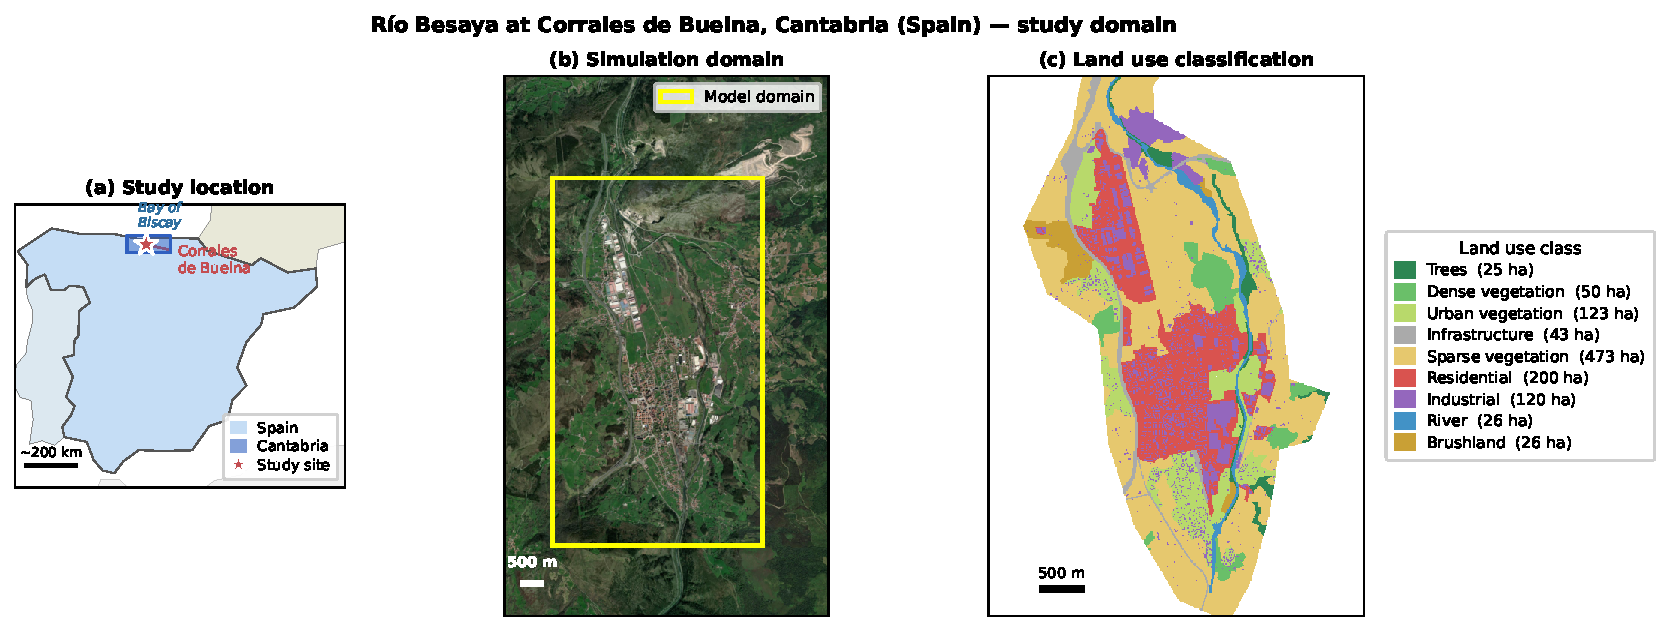
\includegraphics[width=\textwidth]{figures/fig00_location_map.pdf}\caption{Study area and model domain. (a) Regional location of Corrales de Buelna in Cantabria, northern Spain. (b) Satellite view of the 2D simulation domain. (c) CORINE-derived land-use classification used to assign Manning roughness classes.}
  \label{fig:location}
\end{figure}

The analysed reach covers the urban and peri-urban floodplain of Los Corrales de Buelna, approximately 20~km upstream from the river mouth. It is about 4.5~km long and lies at elevations of roughly 55--70~m~a.s.l. in the ETRS89/UTM Zone~30N coordinate system (EPSG:25830). The active channel is typically 20--40~m wide and is incised several metres below the surrounding low terrace. As a result, the main inundation corridor is well defined, but lateral connectivity with adjacent low-lying areas depends on relatively small differences in local topography.

Land use changes markedly across the floodplain. Industrial and light-commercial areas occupy much of the right bank, mixed with residential zones and transport infrastructure. The left bank is more open and vegetated, with riparian woodland, dense gallery vegetation, pasture and brushland. This combination of built-up surfaces, channel margins and vegetated floodplain areas makes the reach suitable for analysing the propagation of spatially distributed Manning roughness uncertainty. In the model domain, sparse vegetation and residential areas are the dominant classes, accounting for approximately 43.6\% and 18.4\% of the mapped area, respectively (Figure~\ref{fig:location}c).

A notable feature of the reach is a secondary low-lying area on the left bank, separated from the main inundation corridor by a local topographic saddle at approximately 60~m~a.s.l. The depression covers about 7.4~ha and lies mainly below the saddle elevation. Its hydraulic connection to the primary floodplain therefore depends on whether water levels at the controlling saddle are exceeded during the event. This topographic configuration is relevant for the interpretation of the ensemble results presented later in the paper, but it is introduced here simply as a geomorphic feature of the study reach.

The Besaya River is gauged at Corrales de Buelna (station A025, MITERD/CHC). The annual maximum peak-flow record indicates a strongly skewed flood regime, consistent with the use of extreme-value methods for design-flow estimation. The reach has experienced several damaging floods, including events in 1983, 2010 and 2019; the 2019 flood caused damage to industrial premises on the right bank. The area is also included in the Spanish \emph{Sistema Nacional de Cartograf\'{\i}a de Zonas Inundables} (SNCZI), which provides regulatory flood-hazard information for several return periods, including the 500-year low-probability scenario. The design event and the basic hydraulic-modelling framework used here build on a previous flood-risk assessment of this reach \citep{navas2018rop}. 

The terrain representation is based on a 5~m resolution digital elevation model derived from airborne LiDAR data acquired by the Spanish Instituto Geográfico Nacional (IGN) in 2018, with a reported vertical RMSE below 0.15~m. The DEM was hydrologically conditioned to remove spurious depressions and preserve channel connectivity. The same conditioned terrain model was used in both hydraulic models so that differences between simulations were not introduced through the elevation input.

Land use was obtained from CORINE Land Cover 2018 and reclassified into nine hydraulically meaningful classes: river, trees, dense vegetation, urban vegetation, sparse vegetation, brushland, residential, industrial and infrastructure surfaces (Figure~\ref{fig:location}c; Table~\ref{tab:manning}). Although CORINE is coarser than the 5~m hydraulic
grid, the reclassified map was checked against 2021 orthophotography to ensure that the main channel, built-up areas, transport corridors and floodplain vegetation were represented consistently at the scale of the model domain. The resulting class map provides the spatial basis for assigning Manning
roughness distributions in the Monte Carlo analysis.

\begin{table}[htbp]
\centering
\caption{Manning roughness coefficient \nman{} by land use class:
bibliographic ranges, sampling distribution (KS-selected as pragmatic choice among three equally plausible candidates), and
Monte Carlo ensemble statistics ($N = 1\,000$).}
\label{tab:manning}
\small
\begin{tabular}{llrccccc}
\toprule
\multirow{2}{*}{Land use class} &
\multirow{2}{*}{Distribution} &
\multirow{2}{*}{Area (\%)} &
\multicolumn{2}{c}{Literature range} &
\multicolumn{3}{c}{MC ensemble} \\
\cmidrule(lr){4-5}\cmidrule(lr){6-8}
& & & $n_{\min}$ & $n_{\max}$ & Mean & Std & CV (\%) \\
\midrule
Trees             & Normal     &  2.3 & 0.100 & 0.250 & 0.165 & 0.047 & 28.5 \\
Dense vegetation  & Normal     &  4.6 & 0.060 & 0.140 & 0.098 & 0.025 & 25.5 \\
Urban vegetation  & Normal     & 11.4 & 0.050 & 0.130 & 0.088 & 0.029 & 32.9 \\
Infrastructure    & Gamma      &  4.0 & 0.011 & 0.020 & 0.015 & 0.003 & 21.2 \\
Sparse vegetation & Gamma      & 43.6 & 0.020 & 0.080 & 0.050 & 0.020 & 39.5 \\
Residential       & Gamma      & 18.4 & 0.010 & 0.020 & 0.015 & 0.004 & 24.7 \\
Industrial        & Gamma      & 11.1 & 0.013 & 0.024 & 0.018 & 0.004 & 20.2 \\
River             & Normal     &  2.3 & 0.025 & 0.060 & 0.040 & 0.011 & 27.2 \\
Brushland         & Gamma      &  2.4 & 0.040 & 0.120 & 0.077 & 0.026 & 33.5 \\
\bottomrule
\end{tabular}
\end{table}



%% ===========================================================================
\section{Methods}
\label{sec:methods}
The methodological workflow follows the same roughness ensemble through two hydraulic model configurations. First, plausible Manning values are sampled for each land-use class and combined into a Monte Carlo ensemble. The same ensemble is then used to run \sfincs{} and \hecras{} under identical terrain, forcing and boundary-condition inputs. The resulting paired simulations are compared at the domain scale and then examined spatially to identify whether any systematic differences between models are associated with specific topographic controls. A final robustness check evaluates how the independence assumption in the Manning sampling affects the main conclusions.

\subsection{Monte Carlo representation of Manning roughness uncertainty}\label{sec:manning_mc}
Manning roughness uncertainty was represented at the level of land-use classes. For each of the nine classes used in the hydraulic models, a set of reference \nman{} values was compiled from standard roughness sources: \citet{chow1959} for the main channel and vegetated floodplain classes, \citet{barnes1967} for natural channel and forested floodplain conditions, \citet{brater1996} for urban and infrastructure surfaces, and \citet{fhwa1984} for composite floodplain roughness. These values were not treated as site measurements, but as empirical support for plausible class-level roughness ranges applicable to the Corrales de Buelna floodplain. Between four and nine values were available for each class, with a median of six. This amount of information is sufficient to define pragmatic sampling distributions for uncertainty propagation, but not to infer detailed distributional shapes with high statistical confidence.

For each land-use class, three candidate parametric distributions were fitted: normal ($\mathcal{N}$), log-normal ($\ln\mathcal{N}$) and gamma ($\Gamma$). Log-normal and gamma distributions ensure strictly positive values, while the normal distribution was also retained as a candidate because, over the roughness ranges considered here, its fitted probability mass below zero was negligible or removed during sampling. These distribution families are commonly used in environmental and hydraulic uncertainty analyses, including roughness-sensitivity studies \citep{pappenberger2005,savage2016}. Parameters were estimated by maximum likelihood using \texttt{scipy.stats.fit}, and the Kolmogorov--Smirnov statistic was used as a selection criterion against the reference values available for each class. The candidate distribution with the highest KS $p$-value was selected for sampling. With only four to nine reference values per class, none of the three families is statistically distinguishable from the others; the selection is therefore a transparent but pragmatic rule, not a statistically definitive result. No candidate was rejected at the 5\% level, which is expected at these sample sizes. The fitted distributions should be interpreted as pragmatic devices for propagating published roughness ranges rather than as validated descriptions of Manning variability.

Sampling was performed in two stages. First, an internal pool of (10,000) positive values was drawn from the selected distribution for each class; negative values, where they occurred for normally distributed classes, were discarded. From this pool, \num{1000} values were then selected without replacement to form the final ensemble for that class. This procedure reduces exact repetition while preserving the empirical shape of the target distribution in the \num{1000}-member ensemble. Combining the nine class-wise samples produced a Manning matrix ($\mathbf{N} \in \mathbb{R}^{1000 \times 9}$), in which each row defines one spatial roughness realisation to be used in both hydraulic models \citep{saltelli2010}.

The class-wise samples were generated independently, with no imposed inter-class correlation. This assumption gives a broad exploration of the plausible roughness space and avoids introducing a dependence structure that cannot be estimated reliably from the available bibliographic values. Its effect on the results is assessed separately in Section~\ref{sec:res_robustness} using the \texttt{generate\_manning\_combinations\_correlated} function of the \texttt{pyhydra} package (\url{https://github.com/navass11/pyhydra}), which implements a Gaussian copula sampler for alternative inter-class correlation structures. The random seed was fixed at 42 to ensure reproducibility. Each of the \num{1000} Manning combinations was also written to an individual CSV file mapping land-use codes to roughness values, so that any hydraulic simulation can be reproduced exactly.


\subsection{Hydraulic model set-up and simulation protocol}\label{sec:model_setup}
The same Manning ensemble was propagated through two 2D hydraulic model configurations: \sfincs{} and \hecras{}. The comparison was designed so that both models used the same terrain source, land-use classes, upstream hydrograph and downstream boundary condition. The two configurations differ, however, in their governing-equation approximation, numerical implementation and mesh representation, and these differences are considered here as part of the broader model-structure effect.

\sfincs{} \citep{deltares2023sfincs,leijnse2021} solves a simplified inertial form of the shallow-water equations. In this formulation, local acceleration and the water- surface pressure gradient are retained, while advective acceleration is neglected. The equations used here can be written as 
\begin{align}
\frac{\partial \eta}{\partial t} + \nabla\cdot(h\mathbf{u}) &= 0 ,
\label{eq:sfincs_cont}\\
\frac{\partial \mathbf{u}}{\partial t} + g\nabla\eta +
\frac{g n^2}{h^{4/3}}\mathbf{u}|\mathbf{u}| &= 0 ,
\label{eq:sfincs_mom}
\end{align}
where $\eta$ is the free-surface elevation, $h = \eta - z_b$ is water depth, $z_b$ is bed elevation, $\mathbf{u}=(u,v)$ is the depth-averaged velocity vector, $g=9.81~\mathrm{m,s^{-2}}$ is gravitational acceleration and \nman is the local Manning roughness coefficient. The simplified inertial approximation is computationally efficient because it avoids the stability constraints associated with the advective momentum terms, allowing larger time steps in many floodplain applications \citep{bates2010}. \sfincs{} was run on a staggered Cartesian grid using its subgrid topography approach, which allows fine-resolution terrain information to be represented within an efficient computational framework. The model domain comprised ($1201 \times 679$) cells at 5~m resolution. All \num{1000} \sfincs{} simulations were executed on GPU
through Docker using Deltares SFINCS v2 and an NVIDIA GeForce RTX 3090.

The \hecras{} configuration used HEC-RAS 6.6 \citep{usace2021hecras} with the full 2D Saint-Venant equations. In contrast to the simplified inertial approximation, this formulation retains the advective acceleration term:
\begin{align}
\frac{\partial \eta}{\partial t} + \nabla\cdot(h\mathbf{u}) &= 0 ,
\label{eq:hecras_cont}\\
\frac{\partial \mathbf{u}}{\partial t} +
\mathbf{u}\cdot\nabla\mathbf{u} + g\nabla\eta +
\frac{g n^2}{h^{4/3}}\mathbf{u}|\mathbf{u}| &= 0 .
\label{eq:hecras_mom}
\end{align}
The term $\mathbf{u}\cdot\nabla\mathbf{u}$ represents advective momentum transport and is relevant where flow acceleration and spatial velocity gradients affect floodplain connectivity, for example near constrictions, embankments or topographic saddles. \hecras{} uses an implicit finite-volume solver on an unstructured mesh. The mesh was derived from the same 5~m DEM used for \sfincs{}, with an average cell-edge length of approximately 25~m in the floodplain and refinement to about 5~m in the main channel. Manning values were assigned through a rasterised land-cover file (\texttt{LandCover.hdf}); for each Monte Carlo realisation, this file was updated programmatically using the \texttt{h5py} library so that the corresponding class-wise roughness values were applied to the \hecras{} mesh.

The forcing event was the $(T=500)$-year flood hydrograph for the Besaya River at Los Corrales de Buelna. The hydrograph was generated with a calibrated HEC-HMS model using the Clark unit hydrograph method for runoff transformation and a Soil Moisture Accounting model for losses, following the HEC-HMS setup described in \citet{navas2018rop}, in which parameters were calibrated to the gauged catchment. The resulting peak discharge at the catchment outlet was $Q_{500}=223~\mathrm{m^3\,s^{-1}}$, consistent with the regionalised frequency analysis of this reach \citep{navas2018rop}. The HEC-HMS hydrograph, originally produced at a 2-minute time step, was resampled to a 1-hour interval for input to both hydraulic models. The simulation window covered 19~days, long enough to include the complete rising limb, peak and recession of the event. At the downstream end of the domain, both models used a normal-depth boundary condition with a bed slope of $S_0=0.001~\mathrm{m,m^{-1}}$, estimated from the 5~m DEM along the channel centreline at the outlet.

Each of the \num{1000} Manning combinations was run once in \sfincs{} and once in \hecras{}, producing a paired hydraulic ensemble. For each simulation, the main output retained for post-processing was the maximum-over-time water-depth raster, \texttt{hamax}. \sfincs{} outputs were already available on the 5~m Cartesian grid, while \hecras{} results were exported to GeoTIFF at 5~m resolution to match the \sfincs{} output grid. The resulting set of \num{2000} GeoTIFF files was managed and analysed in Python using \texttt{xarray} and \texttt{rioxarray}.


\subsection{Flood-output metrics and ensemble cleaning}\label{sec:metrics_cleaning}
The hydraulic response of each simulation was summarised from the maximum-over-time water-depth raster, \texttt{hamax}. The two primary metrics used in the analysis were mean water depth and flooded area. Mean water depth, $\bar{h}$, was computed as the spatial mean of all wet cells, using a wet/dry threshold of $h_{\min}=0.05~\mathrm{m}$, following the convention adopted in large-scale flood-map validation studies \citep{wing2019}. Flooded area, $A$, was computed as the number of wet cells multiplied by the
cell area ($25~\mathrm{m^2}$) and expressed in $\mathrm{km^2}$. Both metrics were calculated at the domain scale rather than at individual cross-sections. This choice reflects the purpose of the ensemble analysis, which is to quantify how roughness uncertainty propagates to overall flood hazard descriptors rather than to calibrate local water levels at gauging points. Local metrics are generally more appropriate for calibration-oriented studies \citep{pappenberger2005,domeneghetti2012}.

Care was taken to compute spatial means directly over the two spatial dimensions at once. Sequential averaging can introduce a small but systematic bias when dry cells are represented as missing values, because the number of valid cells differs between rows or columns. For this reason, dry cells were first masked using the $h_{\min}$ threshold and the mean was then computed as a single reduction over all remaining wet cells.

For each simulation, an effective wet-cell Manning value, $\bar{n}$, was also computed by averaging the reclassified Manning raster over the cells that were wet in that simulation. This value provides a compact summary of the roughness field actually sampled by the inundation and was used as the independent variable in the regression analyses. Because the wet area varies from one realisation to another, $\bar{n}$ is not simply the domain-average roughness; it is conditional on the flood extent produced by each model and each Manning combination.

Two additional metrics were retained to check whether the main results were sensitive to the use of mean depth and flooded area alone. The first was inundation volume, $V$, computed as $V = \bar{h}\times A\cdot10^6$. This combines depth and area in a single scalar and is less affected by the addition or removal of near-dry boundary cells, because cells close to $h_{\min}$ contribute little volume relative to the mean inundation depth. The second was the median wet-cell depth, $\tilde{h}$, which is less sensitive than the arithmetic mean to the sudden inclusion of a large number of shallow cells. These two metrics are used later to test whether the two-regime behaviour observed in the \hecras{} ensemble is a property of the hydraulic response rather than an artefact of the selected summary metric.

Before the statistical analysis, the paired ensemble was screened for numerical non-convergences or unstable simulations. Extreme output values were identified using a robust (z)-score based on the median absolute deviation:
\begin{equation}
z_i^* =
\frac{|x_i - \mathrm{median}(\mathbf{x})|}
{1.4826,\mathrm{MAD}(\mathbf{x})} ,
\label{eq:robust_z}
\end{equation}
where the factor 1.4826 makes the MAD-based scale comparable to the standard deviation under a normal distribution \citep{rousseeuw1993}. A robust statistic was preferred to a classical (z)-score because the latter is itself influenced by the extreme values being detected.

The screening was applied across both models and the two primary flood metrics; a simulation pair was flagged if any metric in either model exceeded $z^*>5$. This threshold was deliberately conservative. A lower threshold, such as $z^*>3$, would risk treating the low-area branch of the \hecras{} bimodal distribution as an anomaly, although it forms part of the hydraulic response analysed in this study. With $z^*>5$, five simulations were removed (indices 29, 295, 633, 724 and 755), corresponding to 0.5\% of the original ensemble. Four of these cases had \hecras{} flooded areas above $1.0~\mathrm{km^2}$ or mean depths above $1.7~\mathrm{m}$, values that were inconsistent with the model-domain geometry; the remaining case had an anomalously low \sfincs{} flooded area. Visual inspection of the corresponding \texttt{hamax} rasters confirmed numerical instability or non-convergent behaviour. Full diagnostics, including the flagged metric, robust (z)-score and outputs from both models, are given in Supplementary Table~\ref{tab:anomalous}. The final dataset therefore consists of $N=\num{995}$ valid paired simulations.


\subsection{Inter-model comparison and sensitivity analysis}\label{sec:sensitivity}
Sensitivity to Manning roughness was first evaluated within each model by relating the effective wet-cell Manning value, $\bar{n}$, to the flood-output metrics defined above. Pearson correlation coefficients were used to measure the strength of the linear association between $\bar{n}$ and each output metric across the $N=\num{995}$ valid simulations. Ordinary least-squares regression was then used to estimate the average change in each output per unit change in $\bar{n}$. Although the relationship between roughness and flood response need not be strictly linear at local scale, this regression provides a simple ensemble-level diagnostic of sensitivity, consistent with the use of screening and diagnostic metrics in environmental-model sensitivity analysis \citep{pianosi2016}.

The spread of each model ensemble was summarised using the coefficient of variation,
\begin{equation}
\CV = \frac{\sigma}{\mu}\times 100 ,
\label{eq:cv}
\end{equation}
where $\mu$ and $\sigma$ are the ensemble mean and standard deviation of the corresponding flood metric. The coefficient of variation was used because the metrics have different units and magnitudes, and because it provides a compact way to compare the relative variability of depth, area and volume across models.

Inter-model consistency was assessed using the paired structure of the ensemble. Each Manning realisation produces one \sfincs{} simulation and one \hecras{} simulation, so the two models can be compared realisation by realisation rather than only through their marginal distributions. Pearson correlation was used to quantify whether simulations producing relatively high or low outputs in one model tended to do the same in the other. Mean bias, computed as the \hecras{} ensemble mean minus the corresponding \sfincs{}
ensemble mean, was used to quantify systematic differences between the models. Root mean square error (RMSE) was computed over paired simulations to summarise the combined effect of systematic offset and simulation-to-simulation disagreement.

The relationship between Manning roughness and the \hecras{} inundation regime identified later in the analysis was evaluated separately. Spearman rank correlations were computed between each individual land-use Manning coefficient and the binary regime label. The same test was also applied to the effective wet-cell Manning value, $\bar{n}$. Differences in Manning values between the two regime groups were assessed using Student's two-sample (t)-test when the distributions were approximately normal, as checked with the Shapiro--Wilk test at $\alpha=0.05$. When this assumption was not met, the Mann--Whitney (U)-test was used instead. All statistical tests were two-tailed and used a
significance level of $\alpha=0.05$.


\subsection{Regime detection and topographic-threshold analysis}\label{sec:regime_threshold}
The \hecras{} flooded-area ensemble showed two visually distinct clusters in the initial exploratory analysis. To formalise this separation, the distribution of flooded area, $A$, was represented with a Gaussian mixture model. A two-component mixture was fitted as
\begin{equation}
p(A) = \sum_{k=1}^{2} \pi_k\,
\mathcal{N}(A;\,\mu_k,\,\sigma_k^2),
\label{eq:gmm}
\end{equation}
where $\pi_k$, $\mu_k$ and $\sigma_k^2$ are the weight, mean and variance of component $k$. Parameters were estimated by Expectation--Maximisation using ten random initialisations and a convergence tolerance of $10^{-6}$. Each simulation was assigned to the component with the highest posterior probability, following a maximum a posteriori classification rule. The choice of two components was based first on the kernel density estimate of flooded area and then checked with the Bayesian Information Criterion, which reached its minimum for $K=2$ and increased for larger mixtures. The resulting classes are referred to as the low- and high-inundation regimes.

The spatial signature of these regimes was examined using inundation-frequency maps. For each regime $k$, a frequency raster $f_k(\mathbf{x})$ was computed as the fraction of simulations in that regime for which cell $\mathbf{x}$ was wet, using the same threshold $h_{\min}=0.05~\mathrm{m}$ as in the flood-metric calculation. The low regime contained 97 simulations. The high regime contained 898 simulations, so its frequency map was computed from a random subset of 80 simulations to reduce computational cost. Tests with subset sizes of $n = 40$, 60 and 80 showed that the spatial pattern stabilised for $n \geq 60$. Across three independent random seeds, 99.9\% of domain cells had an absolute frequency difference $|f_{60} - f_{80}| < 0.05$, and the domain-wide mean absolute difference was below 0.001. Within $\Omega_{\mathrm{secondary}}$ specifically, the mean cell-level difference was below 0.04 and the maximum was below 0.15; the larger values at individual cells occur at the boundary of the secondary compartment where frequency values are near the $f_{\mathrm{high}} = 0.6$ threshold used for the zone definition. These results confirm that 80 simulations were sufficient to characterise the high-regime inundation footprint and to locate the secondary compartment used in the corridor analysis, although the exact boundary of $\Omega_{\mathrm{secondary}}$ may shift by a few cells depending on the subset seed.

The part of the floodplain associated specifically with the high-inundation regime was defined by contrasting the two frequency maps: 
\begin{equation}
\Omega_{\mathrm{secondary}} =
\left\{
\mathbf{x} :
f_{\mathrm{high}}(\mathbf{x}) > 0.6
\;\text{and}\;
f_{\mathrm{low}}(\mathbf{x}) < 0.2
\right\}.
\end{equation}
This definition isolates cells that are frequently wet in the high regime but rarely wet in the low regime, rather than cells that are simply close to the main wet/dry boundary in both cases.

To identify the topographic control connecting this secondary zone to the main inundation corridor, a morphological corridor analysis was applied to the binary inundation masks. The permanently inundated area in the low regime, defined as cells wet in all 97 low-regime simulations, and $\Omega_{\mathrm{secondary}}$ were each dilated by five binary iterations. The candidate corridor was then defined as the intersection of the two dilated masks, excluding the two original zones. Within this corridor, the controlling saddle was taken as the minimum-elevation cell in the 5~m LiDAR DEM reprojected to the model grid. This procedure provides a reproducible way to locate the
lowest topographic connection between the main inundation corridor and the secondary floodplain compartment.




\subsection{Robustness to inter-class roughness correlation}\label{sec:correlation_robustness}
The Monte Carlo ensemble described in Section~\ref{sec:manning_mc} assumes independence between Manning values assigned to different land-use classes. This is a practical assumption, but not necessarily a physical one. Roughness values for vegetation-related classes, for example, may be positively correlated because they respond to common seasonal or maintenance conditions, whereas built-up and vegetated classes may show different forms of dependence. The available bibliographic roughness values are not sufficient to estimate a class-to-class correlation matrix directly, so the effect of this assumption was examined through a controlled sensitivity check rather than by redefining the main ensemble.

Inter-class dependence was represented with a Gaussian copula \citep{nelsen2006} applied to the nine fitted marginal distributions used in the original Monte Carlo sampling. An equicorrelation structure was adopted, so that all pairs of land-use classes share the same correlation coefficient $\rho$. This deliberately simple structure does not attempt to reproduce a site-specific dependence model; its purpose is to test whether the main conclusions are sensitive to plausible increases in the correlation among class-wise roughness values. Correlated Manning combinations were generated with the \texttt{generate\_manning\_combinations\_correlated} function in \texttt{pyhydra}, which maps correlated Gaussian variables to the fitted class-wise Manning distributions through their cumulative distribution functions.

Because rerunning the complete hydraulic ensemble for each correlation scenario would have required a large additional computational effort, the effect of inter-class dependence on the existing results was approximated by importance sampling. Each of the \num{995} valid simulations was assigned a weight proportional to the ratio between the Gaussian-copula density for a given value of $\rho$ and the density under the independent sampling used in the original ensemble. The probability integral transforms of the nine Manning coefficients were estimated empirically from the generated ensemble. Weighted kernel density estimates and weighted regime fractions were then computed for the selected correlation scenarios. The effective sample size was reported in each case to indicate the degree of weight concentration.

This analysis was used only as a robustness check. It does not replace the independent Monte Carlo ensemble used for the hydraulic simulations, and it cannot capture changes that would arise if the hydraulic models were rerun with new correlated roughness realisations. It does, however, provide a diagnostic of whether the observed distributional structure is likely to be an artefact of the independence assumption. Details of the copula construction, weighted distributions and effective sample sizes are provided in the Supplementary Material.

\section{Results and discussion}\label{sec:results_discussion}
The results are presented together with their interpretation because the main findings depend not only on the magnitude of the simulated flood outputs, but also on the structure of the model response. The first part of the section summarises the Manning ensemble and its effect on domain-scale flood metrics. The analysis then turns to the paired comparison between \sfincs{} and \hecras{}, where differences in sensitivity, bias and distribution shape reveal a model-structure effect that is not apparent from mean outputs alone. Particular attention is given to the bimodal \hecras{} response, its relation to a topographic saddle controlling access to a secondary floodplain compartment, and its implications for probabilistic flood-hazard mapping.

\subsection{Manning ensemble and effective roughness variability}\label{sec:res_manning}
Table~\ref{tab:manning} summarises the bibliographic Manning ranges, the selected parametric distributions and the Monte Carlo statistics obtained for each land-use class. The normal distribution was selected for four of the nine classes (trees, dense vegetation, urban vegetation and river); the gamma distribution was selected for the remaining five. For the four normal classes, the seven bibliographic reference values span roughly symmetric ranges around their class means, so the normal distribution attains a higher KS $p$-value than log-normal or gamma when fitted to those few points. As noted in Section~\ref{sec:manning_mc}, all three families are statistically indistinguishable at these sample sizes, so the selected family is a pragmatic outcome of the KS criterion. The ensemble statistics reported in Table~\ref{tab:manning} (mean, standard deviation and CV) were computed directly from the realised Monte Carlo draws stored in the combination matrix, not derived analytically from the fitted distributions; they are therefore fully consistent with the updated distribution labels and unchanged from previously reported values. The largest relative uncertainty occurs in the sparse-vegetation class, with an ensemble coefficient of variation of 39.5\%. This class includes transitional covers such as pasture, fallow land and open vegetated areas, for which published roughness values span a wide range of field conditions. By contrast, infrastructure and residential surfaces show the smallest ensemble variability (CV below 25\%), reflecting the more constrained roughness ranges usually assigned to paved, compacted or built-up areas. The river class has an intermediate variability (CV = 27.2\%), because the bibliographic values cover conditions ranging from relatively smooth gravel-bed reaches to more sinuous channels with vegetated banks.

\begin{figure}[htbp]
  \centering
  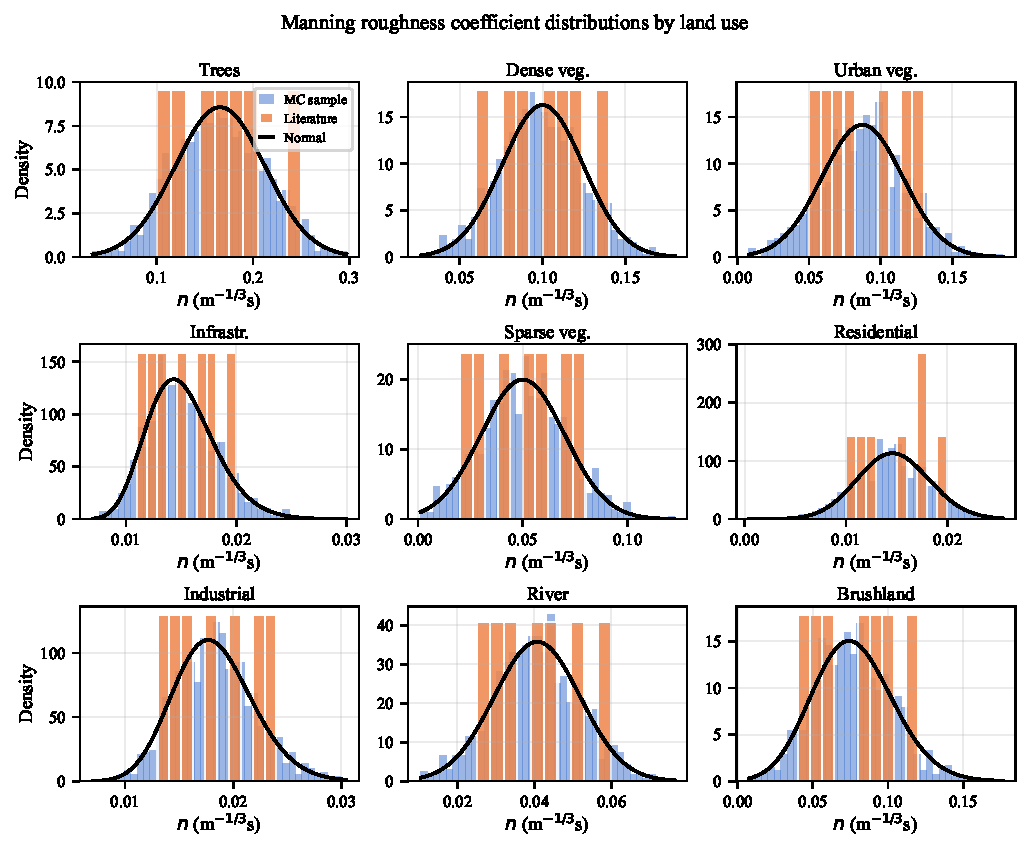
\includegraphics[width=\textwidth]{figures/fig01_manning_distributions.pdf}
 \caption{Class-wise Manning roughness distributions used in the Monte Carlo ensemble. Solid curves show the selected fitted distributions, blue histograms show the sampled values, and orange bars indicate the bibliographic reference values.}\label{fig:distributions}
\end{figure}

The fitted probability density functions and the Monte Carlo histograms are shown in Figure~\ref{fig:distributions}. The close agreement between them indicates that the two-stage sampling procedure, based on an initial pool of (10,000) samples followed by selection of \num{1000} values without replacement, reproduced the intended class-wise distributions. The figure also shows how the shape of each histogram reflects the information contained in the bibliographic values. Classes with tightly grouped reference values, such as infrastructure, generate narrow distributions, whereas classes with more dispersed reference values, such as trees and sparse vegetation, generate broader samples.

\begin{figure}[htbp]
  \centering
  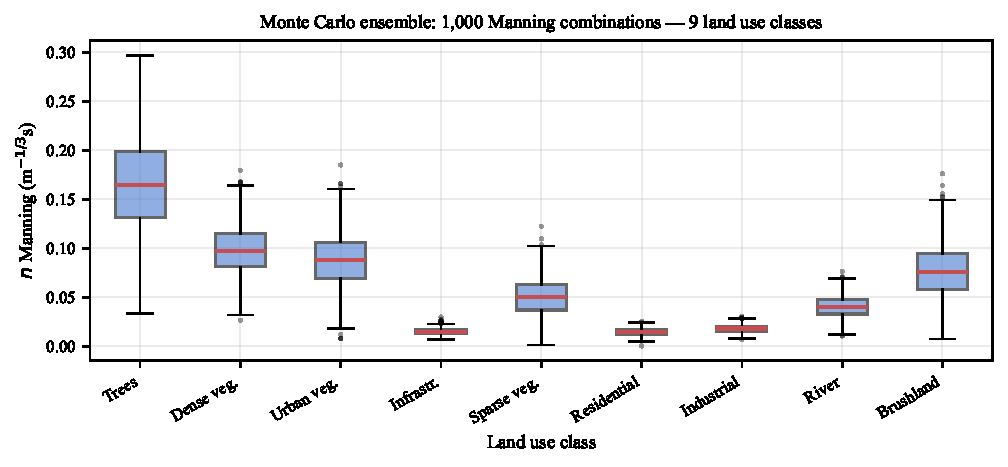
\includegraphics[width=\textwidth]{figures/fig02_mc_boxplots.pdf}
 \caption{Box plots of sampled Manning roughness values for the nine land-use classes across the \num{1000} Monte Carlo combinations. Boxes denote the interquartile range, whiskers extend to $1.5\times\mathrm{IQR}$, and central lines indicate medians.}\label{fig:mc_boxplots}
\end{figure}

Figure~\ref{fig:mc_boxplots} compares the spread of the \num{1000} sampled Manning values across the nine land-use classes. Median values range from about $0.015~\mathrm{m^{-1/3}s}$ for infrastructure and residential areas to about $0.165~\mathrm{m^{-1/3}s}$ for trees, spanning roughly one order of magnitude across the domain. However, the effective Manning value sampled by the inundation is much less variable than the individual classes. Across the \num{995} valid simulations, the spatially averaged wet-cell roughness $\bar{n}_{\mathrm{wet}}$ ranges from approximately $0.026$ to $0.094~\mathrm{m^{-1/3}s}$, with a mean close to $0.059~\mathrm{m^{-1/3}s}$ (wet-cell conditional mean; cf.\ the area-weighted domain average of $0.048~\mathrm{m^{-1/3}s}$ in Table~\ref{tab:manning}, which includes always-dry cells) and a
coefficient of variation of about 18\%. The wet-cell mean exceeds the domain average because the inundation footprint over-represents the rougher vegetated and channel classes that line the active corridor, while always-dry areas are dominated by lower-roughness residential, industrial and infrastructure surfaces. This reduction in variability is a direct consequence of spatial averaging over a heterogeneous floodplain: high- and low-roughness classes are combined within each inundation footprint, and the influence of extreme class values is diluted by the dominant mid-range land-use classes.

No correlation was imposed between Manning values assigned to different land-use classes. The ensemble should therefore be interpreted as a broad exploration of feasible class-level roughness combinations rather than as a set of physically conditioned realisations. The implications of this independence assumption are examined later through the correlated-roughness robustness check.

\subsection{Domain-scale sensitivity to Manning roughness}\label{sec:res_sensitivity}

Figure~\ref{fig:sensitivity} and Table~\ref{tab:sensitivity} summarise the relationship between the spatially averaged wet-cell Manning coefficient, $\bar{n}_{\mathrm{wet}}$, and the main flood-output metrics for the \num{995} valid simulations. At the domain scale, both models show weak direct sensitivity to Manning roughness, although the magnitude and structure of the response differ markedly between them.





\begin{figure}[htbp]
  \centering
  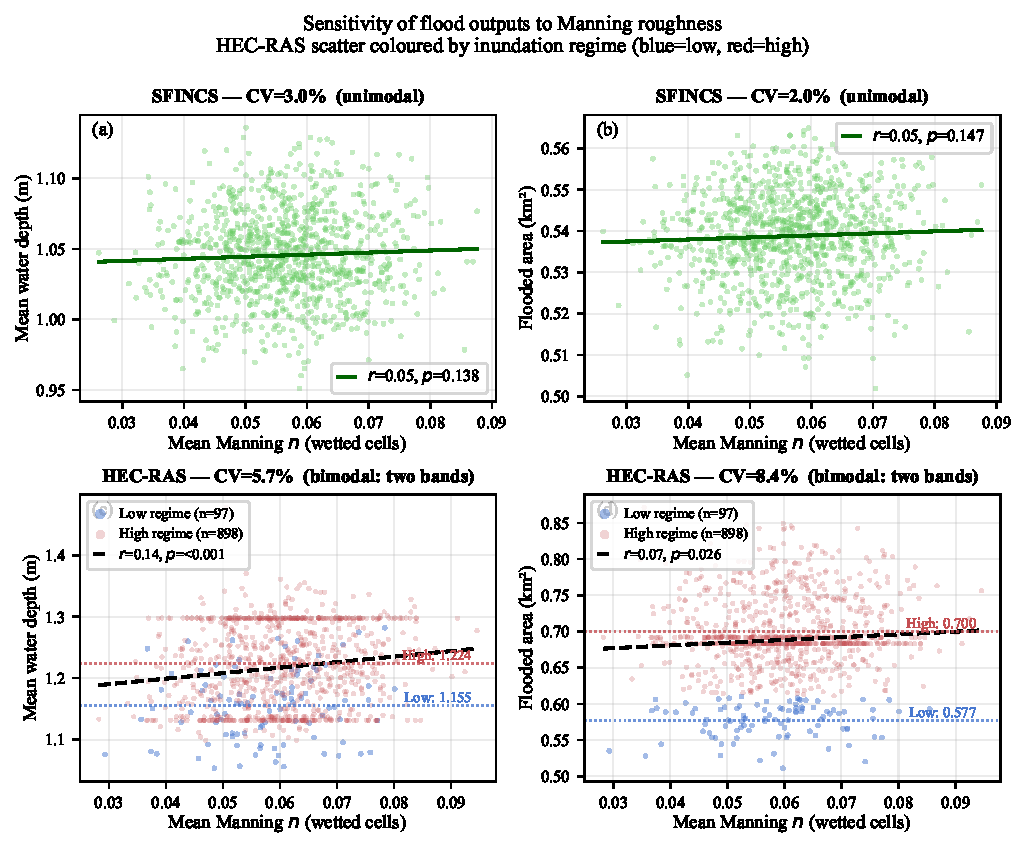
\includegraphics[width=\textwidth]{figures/fig03_intramodel_sensitivity.pdf}\caption{Sensitivity of mean water depth and flooded area to the spatially averaged wet-cell Manning coefficient in \sfincs{} and \hecras{}. Points in the \hecras{} panels are coloured by the GMM-classified inundation regime; horizontal dotted lines mark regime means and dashed lines show linear regressions.}\label{fig:sensitivity}
\end{figure}
\begin{table}[htbp]
\centering \caption{Sensitivity of flood outputs to Manning roughness: Pearson correlation ($r$), coefficient of determination ($r^2$), linear regression slope and coefficient of variation (CV) for each model across 995 valid simulations. $p$-values refer to the test $H_0: r = 0$; n.s.\ = not significant at the 5\% level.}\label{tab:sensitivity}
\footnotesize
\setlength{\tabcolsep}{5pt}
\begin{tabular}{llcccccr}
\toprule
Model & Output metric & Mean & SD & CV (\%) &
$r$ & $r^2$ & Slope$^{a}$ \\
\midrule
\sfincs{}  & Mean depth (m)     & 1.045 & 0.031 & 3.0 & 0.047 (n.s.)      & 0.002 & 0.15 \\
\sfincs{}  & Flooded area (km²) & 0.539 & 0.011 & 2.0 & 0.046 (n.s.)      & 0.002 & 0.05 \\
\hecras{}  & Mean depth (m)     & 1.217 & 0.069 & 5.7 & 0.138 ($p<0.001$) & 0.019 & 0.90 \\
\hecras{}  & Flooded area (km²) & 0.688 & 0.058 & 8.4 & 0.071 ($p<0.05$)  & 0.005 & 0.38 \\
\bottomrule
\multicolumn{8}{l}{$^{a}$ Slope of output on spatially averaged wet-cell Manning $\bar{n}_{\mathrm{wet}}$;
  units: m or km$^2$ per unit of $n$ (m$^{-1/3}$\,s).}
\end{tabular}
\end{table}

For \sfincs{}, the relationship between $\bar{n}_{\mathrm{wet}}$ and the two primary flood metrics is close to negligible. The Pearson correlation is $r=0.047$ for mean water depth ($p=0.14$) and $r=0.046$ for flooded area ($p=0.15$), neither of which is significant at the 5\% level. The ensemble spread is also small, with coefficients of variation of 3.0\% for mean depth and 2.0\% for flooded area. The corresponding regression slopes are $\partial\bar{h}/\partial n = 0.15~\mathrm{m}$ per unit $n$ and
$\partial A/\partial n = 0.05~\mathrm{km^2}$ per unit $n$. In the scatter plots, the \sfincs{} simulations form a continuous and unimodal cloud across the full range of sampled roughness values, with no visible regime structure.

The \hecras{} ensemble is more variable and shows a stronger, although still limited, association with Manning roughness. The Pearson correlation is $r=0.14$ for mean depth ($p<0.001$) and $r=0.07$ for flooded area ($p=0.026$). These correlations are statistically significant, but their practical explanatory power is small: the corresponding $r^2$ values are approximately 0.02 and 0.005, indicating that $\bar{n}_{\mathrm{wet}}$ explains at most 2\% of the variance in the domain-scale outputs. The \hecras{} regression slopes are nevertheless substantially steeper than those obtained with \sfincs{}: $\partial\bar{h}/\partial n = 0.90~\mathrm{m}$ per unit $n$ for mean depth and $\partial A/\partial n = 0.38~\mathrm{km^2}$ per unit $n$ for flooded area. These values are approximately six and eight times larger, respectively, than the corresponding \sfincs{} slopes. The ensemble CVs show the same contrast: 5.7\% for mean depth and 8.4\% for flooded area in \hecras{}, compared with 3.0\% and 2.0\% in \sfincs{}.

A distinctive feature of the \hecras{} scatter plots is that the simulations do not form a single continuous cloud. Instead, flooded area and mean depth are organised into two near-horizontal bands. The lower band contains 97 simulations, with a mean flooded area of $\bar{A}_{\mathrm{low}}=0.577~\mathrm{km^2}$, whereas the upper band contains
898 simulations, with $\bar{A}_{\mathrm{high}}=0.700~\mathrm{km^2}$. The separation between the two bands is therefore $\Delta A \approx 0.124~\mathrm{km^2}$, much larger than the within-band dispersion $\sigma_{\mathrm{low}}=0.023~\mathrm{km^2}$ and $\sigma_{\mathrm{high}}=0.046~\mathrm{km^2}$. Importantly, both bands span almost the full range of $\bar{n}_{\mathrm{wet}}$. The low regime ranges from approximately 0.029 to $0.086~\mathrm{m^{-1/3}s}$, and the high regime from approximately 0.028 to $0.094~\mathrm{m^{-1/3}s}$. Thus, similar effective Manning values can lead to either flooded-area state in \hecras{}. This pattern indicates that the band separation is not simply a direct consequence of mean roughness, but reflects an additional hydraulic or topographic control that is analysed in Section~\ref{sec:res_bifurcation}.

The low explanatory power of Manning roughness at the domain scale is consistent with previous studies showing that roughness uncertainty often has a stronger effect near floodplain margins or locally sensitive areas than on spatially averaged flood metrics \citep{aronica2002,hall2005,fewtrell2011, savage2016}. In the present case, two factors help explain this behaviour. First, the outputs are aggregated over approximately $2.1\times10^4$ to $2.8\times10^4$ wet cells per simulation, which buffers local roughness
signals. Second, the effective wet-cell Manning value has a much narrower relative spread than the individual land-use classes. For \hecras{}, $\bar{n}_{\mathrm{wet}}$ has a coefficient of variation of about 18\% and a 5th--95th percentile range of approximately $0.040$--$0.077~\mathrm{m^{-1/3}s}$, whereas the individual class CVs range from about 20\% to 40\%. High-roughness and low-roughness classes therefore influence the inundation footprint, but their effect is diluted by spatial averaging and by the dominant mid-range land-use classes.

The apparently larger \hecras{} sensitivity should also be interpreted with care. Its overall flooded-area CV of 8.4\% includes the variance associated with the separation between the two bands. Within each regime, the area variability is more modest, with CVs of approximately 3.3\% in the low regime and 6.6\% in the high regime. These values are closer to the \sfincs{} spread than the overall \hecras{} CV would suggest. The elevated domain-scale variability in \hecras{} is therefore not only a direct roughness response; it also reflects the presence of a threshold-like change in floodplain connectivity. These differences indicate that the hydraulic model used to propagate Manning
uncertainty is not a neutral component of the uncertainty analysis: it affects both the magnitude of the simulated variability and the form taken by that variability.

\subsection{Inter-model differences and model-structure effects}\label{sec:res_intermodel}
The paired structure of the ensemble allows the two models to be compared simulation by simulation, using exactly the same \num{995} Manning realisations. Figure~\ref{fig:comparison} and Table~\ref{tab:intermodel} show that \hecras{} produces systematically larger flood outputs than \sfincs{}. The mean bias is $+0.172~\mathrm{m}$ for water depth ($\mathrm{RMSE}=0.182~\mathrm{m}$) and $+0.149~\mathrm{km^2}$ for flooded area ($\mathrm{RMSE}=0.158~\mathrm{km^2}$). Expressed as ratios, the mean \hecras{} outputs are 1.17 times larger for depth and 1.28 times larger for area.


\begin{figure}[htbp]
  \centering
  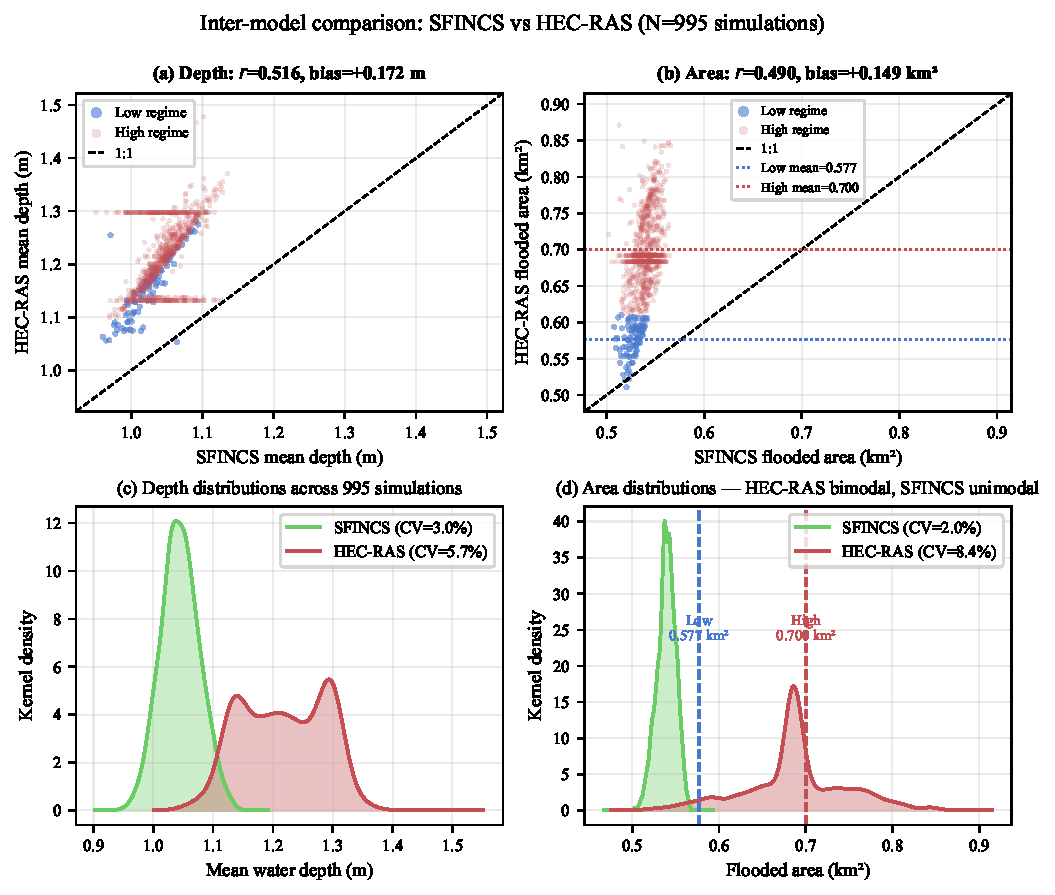
\includegraphics[width=\textwidth]{figures/fig04_intermodel_comparison.pdf}
  \caption{Inter-model comparison of paired \sfincs{} and \hecras{} simulations.
Panels (a--b) show 1:1 comparisons of mean water depth and flooded area, with
dashed lines indicating perfect agreement. Panels (c--d) show the corresponding
ensemble distributions; points are coloured by the \hecras{} inundation regime.}
\label{fig:comparison}
\end{figure}


\begin{table}[htbp]
\centering
\caption{Inter-model comparison metrics (\sfincs{} vs.\ \hecras{}, $N = 995$ paired simulations). Bias = mean(\hecras{}) $-$ mean(\sfincs{}). Ratio = mean(\hecras{}) / mean(\sfincs{}).} \label{tab:intermodel}
\small
\begin{tabular}{lccccc}
\toprule
Output metric & Pearson $r$ & $r^2$ & Bias & RMSE & Ratio \\
\midrule
Mean depth (m)       & 0.52 & 0.27 & $+0.172$~m   & 0.182~m   & 1.17 \\
Flooded area (km²)   & 0.49 & 0.24 & $+0.149$~km² & 0.158~km² & 1.28 \\
\bottomrule
\end{tabular}
\end{table}

The two models are only moderately consistent at the realisation scale. The Pearson correlation between paired simulations is $r=0.52$ for mean depth ($p<10^{-68}$) and $r=0.49$ for flooded area ($p<10^{-60}$). These values indicate that only about one quarter of the inter-simulation variance is shared between the two model ensembles ($r^2=0.27$ for depth and $r^2=0.24$ for area). In practical terms, a Manning combination that produces a relatively large flood in \sfincs{} does not necessarily produce a similarly large flood in \hecras{}. The stochastic roughness field is therefore filtered differently by the two hydraulic configurations.

This difference is visible not only in the mean outputs, but also in the shape of the output distributions. The \sfincs{} flooded-area distribution is unimodal and relatively narrow, with $\bar{A}=0.539~\mathrm{km^2}$ and $\mathrm{CV}=2.0\%$. By contrast, the \hecras{} flooded-area distribution is bimodal, with modes centred near 0.577 and $0.700~\mathrm{km^2}$, and an  overall coefficient of variation of 8.4\%. The 1:1 scatter plots in Figure~\ref{fig:comparison} show the same asymmetry: \sfincs{} varies continuously along the horizontal axis, whereas the \hecras{} area values fall into two distinct clusters. This confirms that the bimodality is not a property of the Manning ensemble itself, but emerges from the way the \hecras{} configuration transforms that ensemble into flood extent.

The systematic positive bias of \hecras{} relative to \sfincs{} is consistent with the interpretation that the full 2D Saint-Venant formulation, together with the numerical and mesh representation used in \hecras{}, allows greater lateral spreading into the floodplain than the simplified inertial configuration used in \sfincs{}. Similar differences between full Saint-Venant and simplified inertial or reduced-complexity models have been reported in estuarine and large-domain applications, where full-momentum models tended to predict larger or more dynamically connected inundation patterns \citep{kumbier2019,vandaele2024}. The comparison made here does not isolate the governing equations alone: it also includes differences in numerical implementation and mesh design. For that reason, the term model-structure effect is used in a broad sense, covering hydraulic formulation, solver implementation and spatial discretisation. In this sense, the inter-model spread is larger than the intra-model spread generated by the Manning ensemble alone. The result is not simply that one model predicts slightly more flooding than the other, but that the hydraulic model is not a neutral component in parameter-uncertainty propagation: the same roughness ensemble is transformed into qualitatively distinct output distributions by the two configurations.

These results reinforce a point that is sometimes obscured in parameter-based uncertainty analyses. The uncertainty associated with Manning roughness is not independent of the model used to propagate it. Here, a narrow unimodal distribution emerges from the \sfincs{} configuration while the same 995-member roughness ensemble yields a wider, bimodal distribution from \hecras{}. The inter-model spread is larger than the within-model spread generated by Manning perturbations alone, which suggests that model structure should be treated as an explicit uncertainty axis in probabilistic flood modelling rather than as a fixed modelling choice made before the uncertainty analysis \citep{teng2017}. For applications such as hazard mapping, emergency planning or design-flood assessment, this distinction is not only methodological: a mean area difference of about 28\% would substantially alter the spatial footprint of the resulting flood-hazard map.



\subsection{Bimodal HEC-RAS response and topographic threshold}\label{sec:res_bifurcation}
The two-band structure observed in the \hecras{} scatter plots corresponds to a bimodal distribution of flooded area. This behaviour was formalised with the two-component Gaussian mixture model described in Section~\ref{sec:regime_threshold}. The model converged in fewer than 15 EM iterations and separated the ensemble into a low-inundation regime, containing 97 simulations ($\pi_0=0.097$), and a high-inundation regime, containing 898 simulations ($\pi_1=0.903$). The fitted mean flooded areas were $\mu_0=0.577~\mathrm{km^2}$ and $\mu_1=0.700~\mathrm{km^2}$, with standard deviations of $0.023~\mathrm{km^2}$ and $0.046~\mathrm{km^2}$, respectively. The difference between the two component means, $\Delta\mu=0.123~\mathrm{km^2}$, is large relative to the within-regime spread, corresponding to $5.4\sigma_0$ and $2.7\sigma_1$. Adding a third component did not improve the Bayesian Information Criterion, confirming that two components are sufficient to describe the observed distribution (Table~\ref{tab:gmm}).

\begin{table}[htbp]
\centering
\caption{GMM-classified inundation regimes for \hecras{} flooded area
($N = 995$). \sfincs{} shows no bimodal structure.}
\label{tab:gmm}
\small
\begin{tabular}{lccccc}
\toprule
Regime & $N$ & $\pi$ (\%) & $\bar{A}$ (km²) & $\sigma$ (km²) & CV (\%) \\
\midrule
Low  (HEC-RAS) &  97 &  9.7 & 0.577 & 0.023 & 4.0 \\
High (HEC-RAS) & 898 & 90.3 & 0.700 & 0.046 & 6.6 \\
\midrule
SFINCS (all)   & 995 & 100  & 0.539 & 0.011 & 2.0 \\
\bottomrule
\end{tabular}
\end{table}


The regime separation is not explained by any single Manning coefficient, nor by the spatially averaged wet-cell roughness. Spearman rank correlations between the nine individual land-use Manning values and the binary regime label are all small and non-significant ($|\rho|<0.03$, $p>0.35$; Table~\ref{tab:regime_manning}). The same is true for $\bar{n}_{\mathrm{wet}}$, for which $\rho=0.014$ and $p=0.66$. One subtlety worth noting is that $\bar{n}_{\mathrm{wet}}$ is computed over the cells that are wet in each realisation, so high-regime simulations --- which additionally wet the secondary compartment --- have more cells in the denominator than low-regime ones. This circularity means that part of the weak $\bar{n}_{\mathrm{wet}}$--regime correlation may reflect the change in averaging domain rather than a genuine absence of roughness control; a domain-wide unconditional average would avoid this but would weight always-dry areas equally. Two-sample tests also show no significant differences in class-wise Manning values between the low- and high-regime groups. These results rule out a simple interpretation in which one roughness class, or the mean roughness of the flooded area, directly controls the transition between regimes. 

\begin{table}[htbp]
\centering
\caption{Spearman rank correlation between individual Manning coefficients
and the \hecras{} inundation regime label (0 = low area, 1 = high area).
No coefficient is significant at the 5\% level ($\alpha = 0.05$),
confirming that no individual Manning coefficient directly explains the regime transition.}
\label{tab:regime_manning}
\small
\begin{tabular}{lcc}
\toprule
Land use class & Spearman $\rho$ & $p$-value \\
\midrule
Trees             & $+0.027$ & 0.394 \\
Dense vegetation  & $+0.002$ & 0.947 \\
Urban vegetation  & $+0.017$ & 0.587 \\
Infrastructure    & $-0.003$ & 0.923 \\
Sparse vegetation & $+0.009$ & 0.770 \\
Residential       & $-0.005$ & 0.869 \\
Industrial        & $<0.001$ & 0.998 \\
River             & $-0.001$ & 0.980 \\
Brushland         & $+0.023$ & 0.477 \\
Mean $\bar{n}$ (wet cells) & $+0.014$ & 0.660 \\
\bottomrule
\end{tabular}
\end{table}


A different picture emerges when the \sfincs{} flooded area for the same Manning realisation is used as a diagnostic. Although the relationship is not strong enough to predict regime membership deterministically, it is statistically significant: the Spearman correlation between \sfincs{} flooded area and the \hecras{} regime label is $\rho=0.3634$ ($p<10^{-31}$). Low-regime \hecras{} simulations are associated with slightly smaller \sfincs{} flooded areas on average ($0.527~\mathrm{km^2}$, compared with $0.540~\mathrm{km^2}$ for high-regime simulations; $t=-12.6$, $p<10^{-30}$). This suggests that the transition is linked to the overall hydraulic state generated by the full roughness field, rather than to any individual class value. Simulations with slightly lower floodplain activation in \sfincs{} are less likely to achieve hydraulic continuity across the saddle corridor in \hecras{}, even though the two models share the same Manning input and boundary conditions.

The spatial frequency maps clarify the source of this regime separation (Figure~\ref{fig:bifurcation}). The high-regime simulations inundate a secondary floodplain compartment on the left bank that is largely absent from the low-regime simulations. This area, $\Omega_{\mathrm{secondary}}$, covers approximately 7.4~ha and is wet in
more than 60\% of the high-regime simulations but in less than 20\% of the low-regime simulations. The frequency-difference map shows a sharp spatial contrast between this compartment and the surrounding terrain, indicating that the regime shift is not a diffuse change along the flood margin but the activation of a coherent secondary inundation area.

\begin{figure}[p]
  \centering
  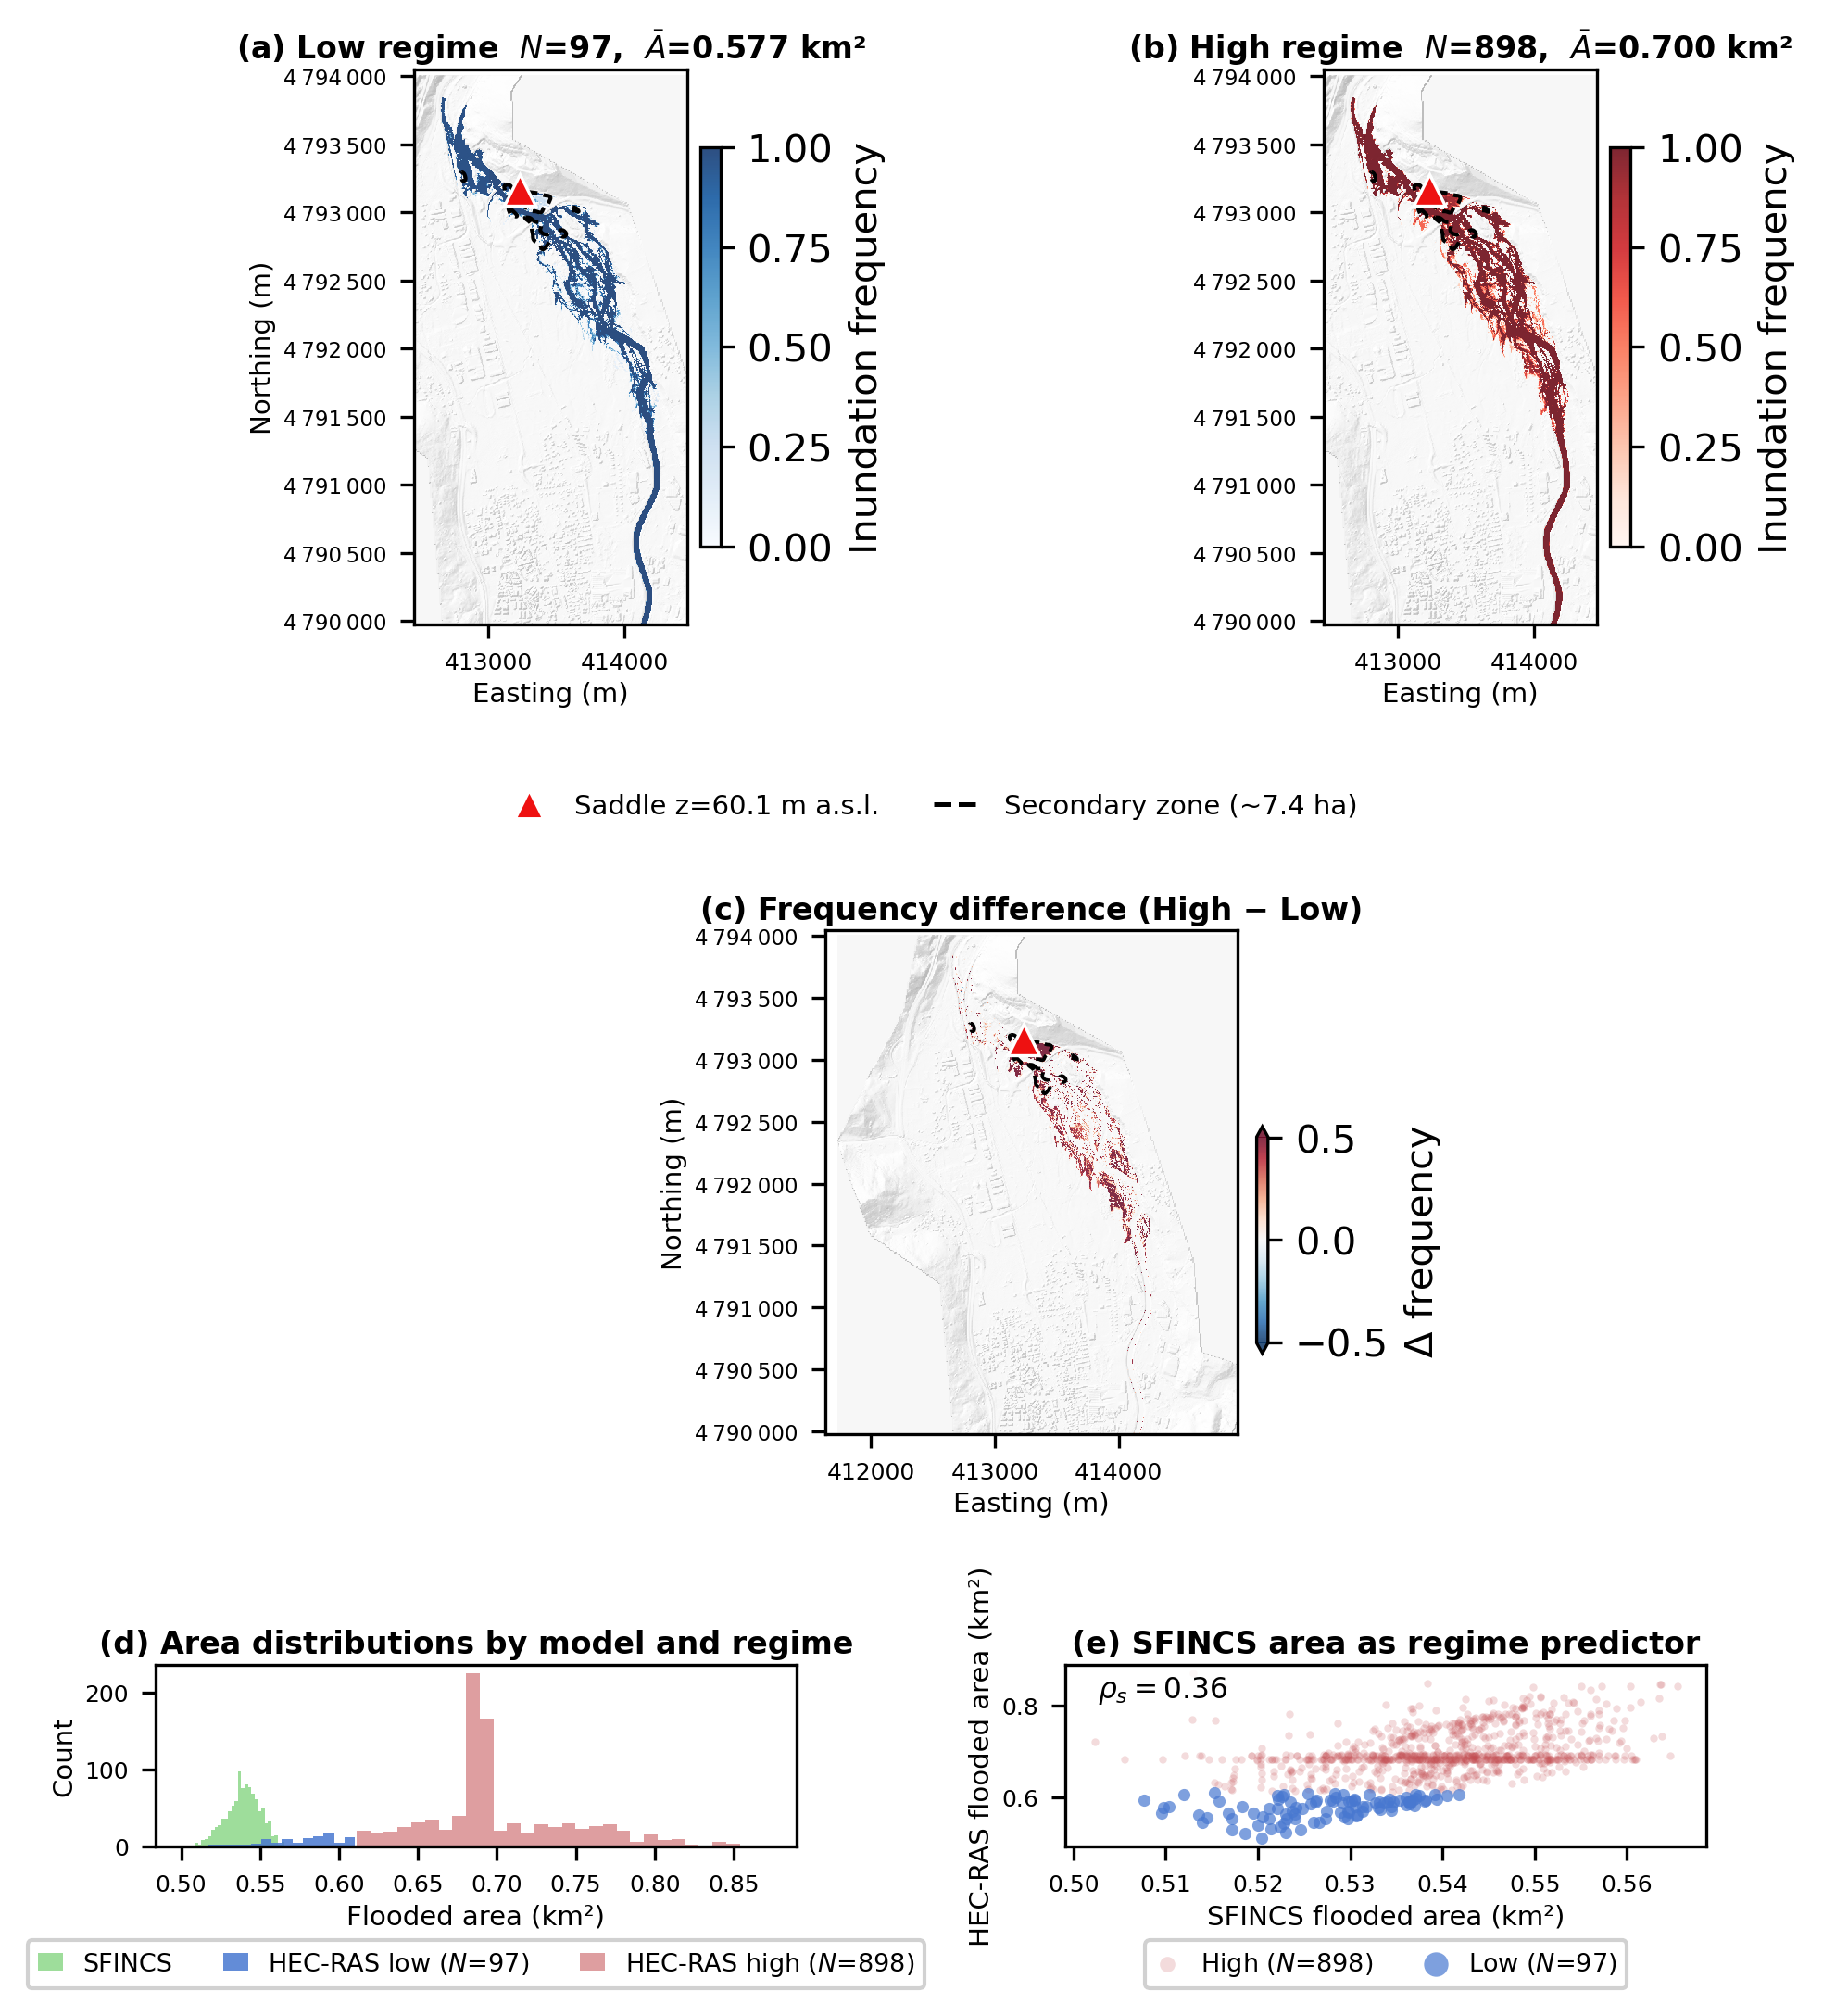
\includegraphics[width=\textwidth]{figures/fig05_hydraulic_bifurcation.pdf}
  \caption{Spatial and distributional evidence of the \hecras{} regime separation. Panels (a--b) show inundation-frequency maps for the low- and high-area regimes, with the secondary floodplain compartment and controlling topographic saddle indicated. Panel (c) shows the frequency difference between regimes, panel (d) compares flooded-area distributions, and panel (e) relates \sfincs{} flooded area to the \hecras{} regime classification.}
  \label{fig:bifurcation}
\end{figure}

The morphological corridor analysis identifies the controlling connection between the main inundation corridor and $\Omega_{\mathrm{secondary}}$ as a topographic saddle at $z=60.1~\mathrm{m}$ a.s.l.\footnote{EPSG:25830 coordinates: X\,=\,413230, Y\,=\,4793166.} The elevation distribution within $\Omega_{\mathrm{secondary}}$ ranges from low-lying depression cells to higher approach slopes, with the lower percentiles corresponding to the depression floor and the upper percentiles to marginal cells that become wet after connection is established. The spatial pattern therefore supports a hydraulic-connectivity interpretation: the secondary compartment becomes activated only when flow conditions across the saddle corridor provide sufficient hydraulic continuity into the adjacent depression.

This compound-connectivity pattern explains the near-horizontal bands in the \hecras{} scatter plots. Once hydraulic continuity across the saddle corridor is established, the secondary compartment is activated as a spatially coherent unit rather than through a gradual expansion of the main flood boundary. The compartment itself accounts for approximately 7.4~ha of additional flooded area, and additional cells are wetted along the connecting corridor and adjacent margins, giving an observed inter-regime difference of about $0.123~\mathrm{km^2}$. The same activation also affects mean depth. The newly connected cells are relatively shallow compared with the pre-existing wet area, so their sudden inclusion changes the wet-cell mean and produces a corresponding band structure in the depth scatter. This behaviour is therefore consistent with a discrete wet/dry transition controlled by local topography, rather than with a continuous response to increasing roughness.

The hydraulic mechanism responsible for the regime-transition behaviour is not fully resolved, but the contrasting responses are consistent with differences in how the two complete model configurations represent flow conditions near the saddle. The \hecras{} configuration combines the full 2D Saint-Venant equations, which retain advective momentum terms ($\mathbf{u}\cdot\nabla\mathbf{u}$), with an unstructured mesh that is coarser in the floodplain ($\sim$25~m) than the 5~m Cartesian grid used by \sfincs{}. Both aspects may contribute to the contrasting connectivity behaviour: the advective terms allow lateral momentum transport towards the saddle that is absent in the simplified inertial formulation, while the coarser floodplain mesh may represent the saddle geometry and connecting corridor differently from the 5~m Cartesian grid. Isolating the relative contribution of these two factors would require an additional controlled experiment --- for example, running \hecras{} with a 5~m structured grid or in diffusion-wave mode on the same mesh --- and is identified as a priority for future work (Section~\ref{sec:limitations}). In the present study, both factors are inseparable components of what is referred to as the model-structure effect. Under some roughness combinations, the flow conditions in the \hecras{} configuration appear sufficient to allow connection to the secondary compartment; under others, hydraulic continuity is not achieved. Because the transition depends on the compound effect of the full roughness field, local velocities, water-surface gradients and the saddle geometry, it is not captured by a single Manning coefficient or by $\bar{n}_{\mathrm{wet}}$. In the \sfincs{} configuration, the combination of the simplified inertial formulation and the regular 5~m grid produces a smoother, unimodal response and does not activate the same secondary compartment as a discrete regime.

This interpretation is supported by three pieces of evidence: the sharply defined frequency contrast around $\Omega_{\mathrm{secondary}}$, the identification of a single topographic saddle controlling hydraulic access, and the partial predictive value of the \sfincs{} flooded area as a proxy for the overall hydraulic state of each realisation. Figure~\ref{fig:saddle_transect} provides direct hydraulic evidence. Panel~(a) shows the maximum inundation extents of one representative low-regime simulation (sim~41, $A = 0.577~\mathrm{km^2}$) and one representative high-regime simulation (sim~132, $A = 0.700~\mathrm{km^2}$), together with the $\Omega_{\mathrm{secondary}}$ boundary. Panel~(b) shows the distribution of maximum water-surface elevation (WSE) at the 5~m DEM pixel coinciding with the morphological saddle ($z = 60.1~\mathrm{m}$ a.s.l.) for all 97 low-regime and all 898 high-regime ensemble members. Both regimes are wet at the saddle pixel in every simulation, with maximum WSE approximately 2~m above the terrain at that location. However, the two regime ensembles exhibit clearly distinct WSE distributions at the saddle: the low-regime ensemble has a median of 62.2~m (IQR: 62.1--62.4~m), whereas the high-regime ensemble has a median of 63.1~m (IQR: 62.5--63.3~m). The two representative simulations fall within their respective regime distributions, with WSE$_{\mathrm{low}}=61.96$~m and WSE$_{\mathrm{high}}=62.92$~m at the saddle. This ${\sim}0.9~\mathrm{m}$ inter-regime difference in WSE at the saddle is consistent with the saddle acting as the control point of a compound hydraulic-connectivity transition: a higher WSE at the saddle is associated with greater hydraulic continuity into the topographic depression that defines $\Omega_{\mathrm{secondary}}$. The two distributions overlap in their tails, however, so that some low-regime members attain a saddle WSE above the lower quartile of the high-regime ensemble, and vice versa. This overlap does not contradict the threshold interpretation: regime labels are assigned by the GMM classifier from the domain-scale flooded-area distribution, not from the local WSE at a single pixel, so boundary-case simulations exist in which the saddle WSE alone does not predict regime membership. The saddle elevation is therefore a necessary but not sufficient condition for secondary-compartment activation; whether hydraulic continuity is established across the connecting corridor depends on the compound flow conditions — velocity gradients, water-surface slopes and the full spatial roughness field — not solely on the magnitude of the local water surface.

\begin{figure}[htbp]
  \centering
  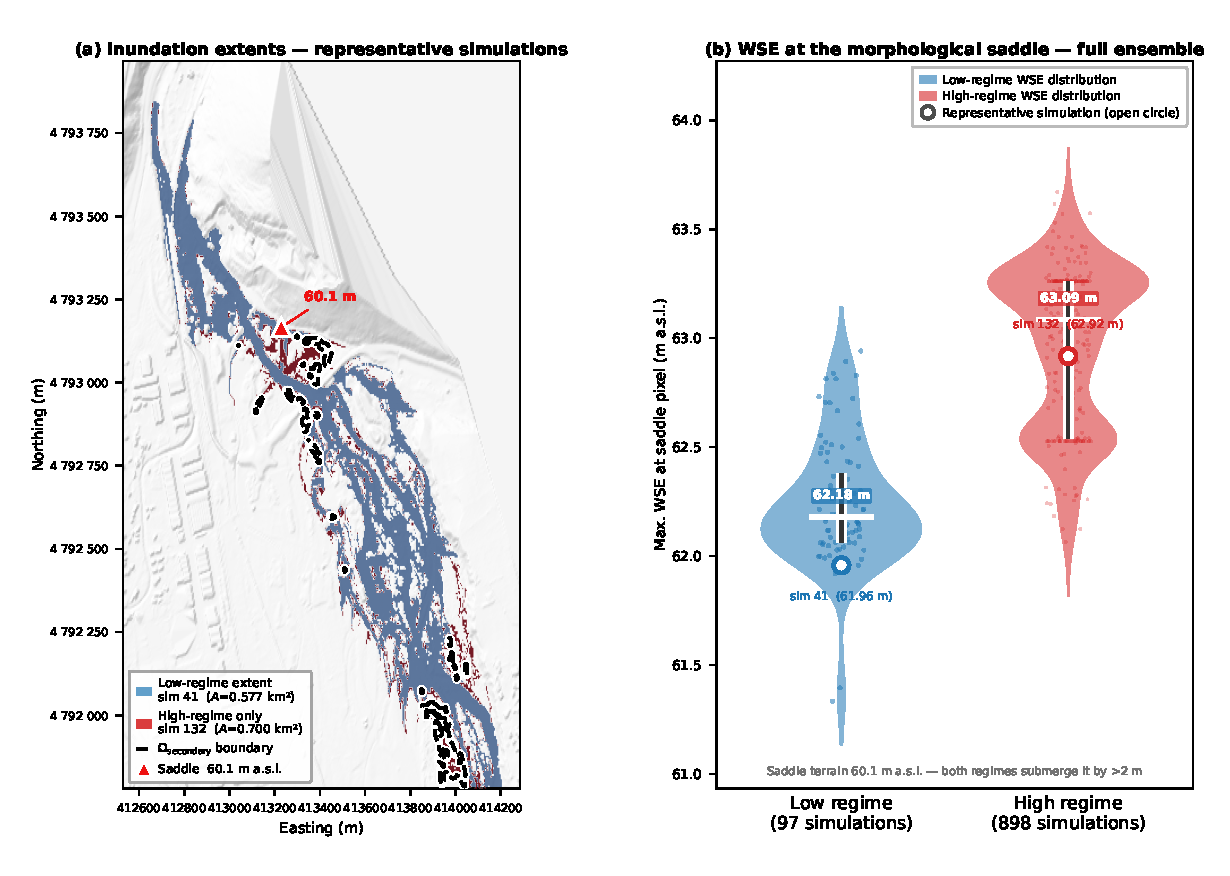
\includegraphics[width=\textwidth]{figures/fig_saddle_transect.pdf}
  \caption{Hydraulic evidence for compound-connectivity regime separation at the morphological saddle.
  (a)~Maximum inundation extents for two representative \hecras{} simulations chosen as the ensemble members whose flooded area is closest to the mean of each regime.
  \textit{Blue fill}: cells inundated in the low-regime simulation (sim~41, $A=0.577~\mathrm{km^2}$), covering the main channel and adjacent floodplain.
  \textit{Red fill}: cells that are wet in the high-regime simulation (sim~132, $A=0.700~\mathrm{km^2}$) but dry in sim~41 --- these additional cells correspond almost entirely to the secondary floodplain compartment.
  The \textit{black dashed contour} (with white outline for visibility) delineates $\Omega_{\mathrm{secondary}}$, defined as the set of pixels whose inundation frequency exceeds 0.6 in the high-regime sub-ensemble and is below 0.2 in the low-regime sub-ensemble.
  The \textit{red triangle} marks the morphological saddle at $z=60.1~\mathrm{m}$ a.s.l., the minimum-elevation connection between the always-wet zone and $\Omega_{\mathrm{secondary}}$.
  (b)~Maximum water-surface elevation (WSE $=$ depth $+$ terrain) at the 5~m DEM pixel coinciding with the morphological saddle, extracted from every simulation in each regime.
  \textit{Violin shapes} are kernel density estimates of the WSE distribution; each violin is overlaid with the individual simulation values (jittered horizontally for visibility; for the high regime, a random subsample of 250 out of 898 points is shown).
  The \textit{central vertical bar} spans the interquartile range (Q1--Q3) and the \textit{horizontal tick} marks the median.
  \textit{Coloured labels} inside each violin report the median WSE (62.18~m for the low regime; 63.09~m for the high regime).
  \textit{Open circles} identify the two representative simulations (sim~41 at 61.96~m; sim~132 at 62.92~m).
  The note at the base of the panel shows the saddle terrain elevation ($z=60.1~\mathrm{m}$ a.s.l.) for reference.}\label{fig:saddle_transect}
\end{figure}

\subsection{Robustness of the bifurcation to alternative metrics and correlated roughness}\label{sec:res_robustness}
The preceding analysis was based mainly on mean water depth and flooded area. These are standard flood-hazard descriptors, but both can be affected by the wet/dry threshold used to define inundated cells. To check whether the \hecras{} regime separation was an artefact of these particular metrics, the sensitivity analysis was repeated using median wet-cell depth, $\tilde{h}$, and inundation volume, $V$ (Figure~\ref{fig:alt_metrics}).

\begin{figure}[htbp]
  \centering
  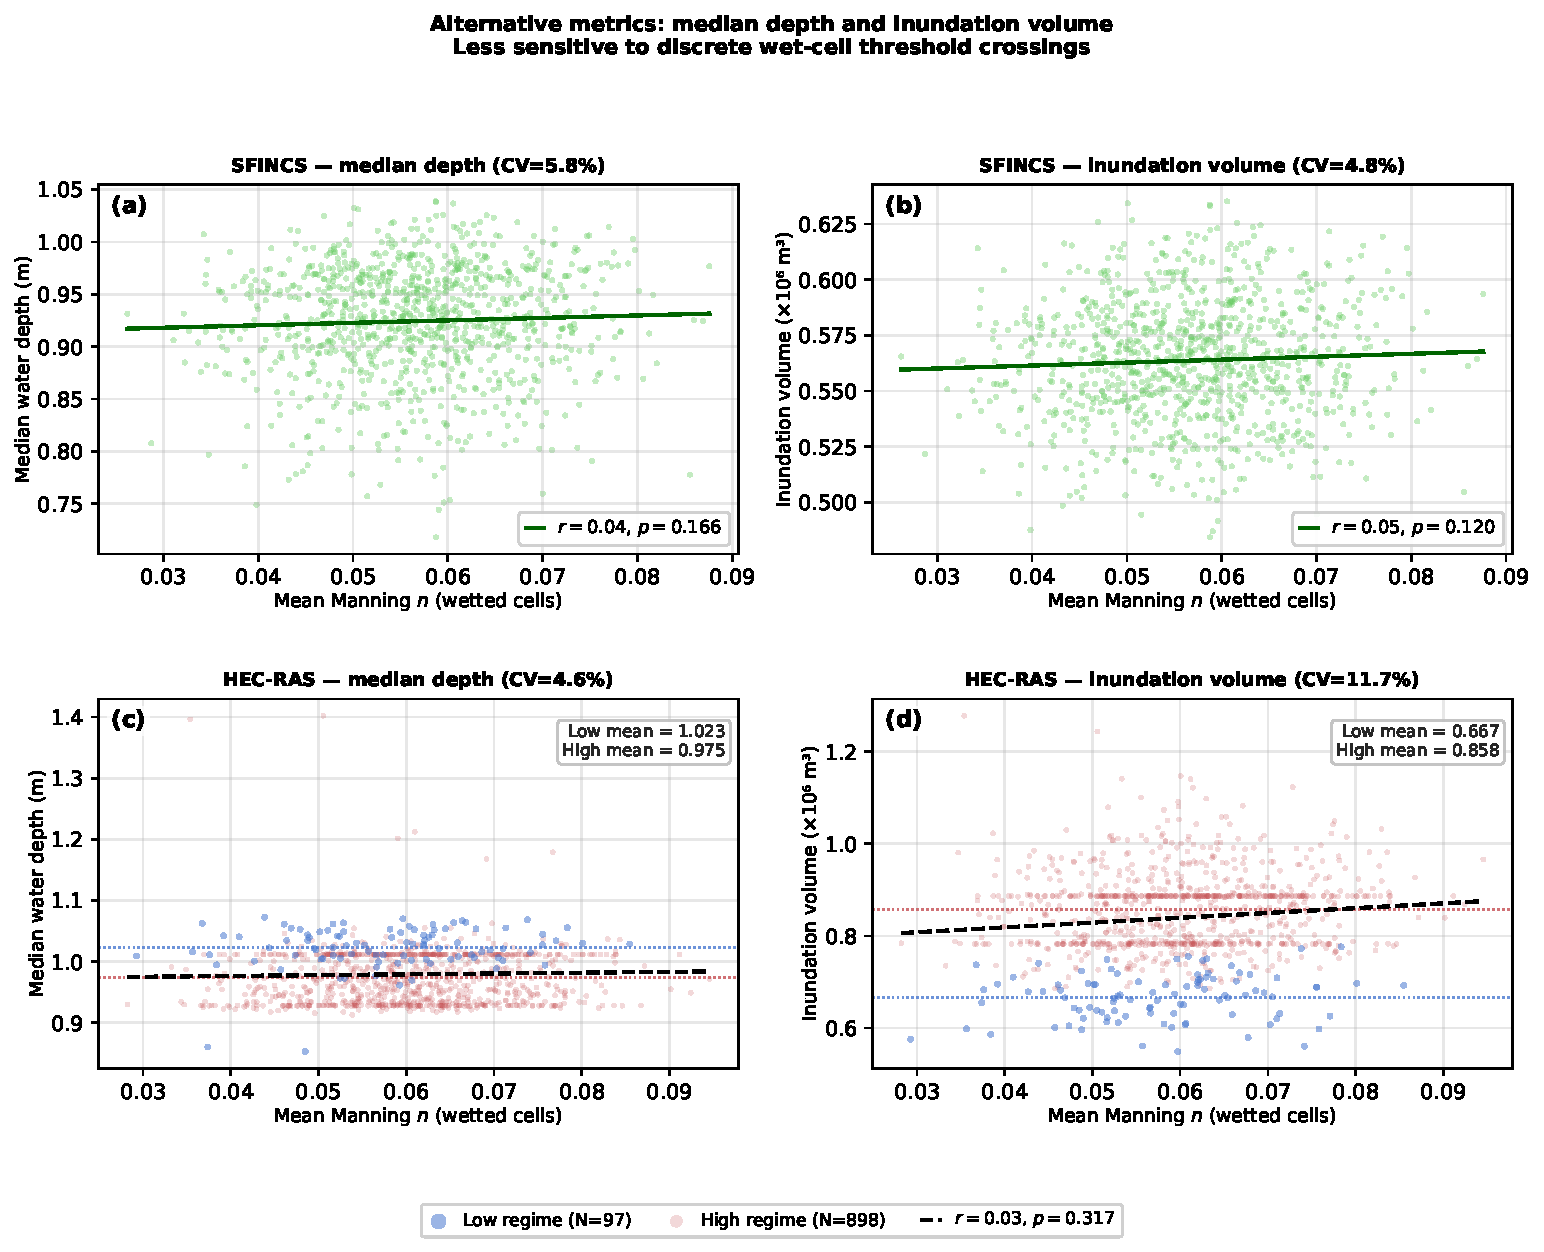
\includegraphics[width=\textwidth]{figures/fig07_alternative_metrics.pdf}
  \caption{Sensitivity analysis using alternative flood-output metrics. Panels show median wet-cell depth and inundation volume as functions of the spatially averaged wet-cell Manning coefficient for \sfincs{} and \hecras{}. \hecras{} points are coloured by inundation regime; dashed lines show linear regressions.}\label{fig:alt_metrics}
\end{figure}

The median-depth results show that the two-regime structure is much less pronounced when the output is based on a robust central tendency. The coefficient of variation of median depth is 5.8\% in \sfincs{} and 4.6\% in \hecras{}. This differs from the behaviour of the mean-depth metric, for which \hecras{} was more variable than \sfincs{}. In \sfincs{}, the median is more sensitive than the mean because the wet-cell boundary shifts gradually with roughness: as marginal cells fall below $h_{\min}$, the depth distribution of the remaining wet cells changes even when the spatial mean is buffered. In \hecras{}, by contrast, the regime transition adds many shallow cells to the wet domain. These cells affect the arithmetic mean more strongly than the median, so the gap between the two \hecras{} regimes is compressed in the median-depth scatter. Median depth is therefore useful for separating within-regime depth variability from changes driven by the sudden inclusion of near-threshold cells.

The volume metric leads to a different but complementary conclusion. The coefficient of variation of inundation volume is 4.8\% in \sfincs{} and 11.7\% in \hecras{}, and the \hecras{} volume scatter retains the two-band structure. This indicates that the bimodality is not an artefact of flooded area alone, nor of the way the wet-cell mean depth is computed. At the same time, the relative jump in volume is smaller than the jump in area. At the moment of activation, the secondary compartment contributes at most $h_{\min}\Delta A = 0.05 \times 74,000 \approx 3700~\mathrm{m^3}$, which is only about 0.5\% of the typical total inundation volume ($\bar{V}\approx 820,000~\mathrm{m^3}$). The secondary floodplain therefore has a strong effect on area-based hazard classification, but a more limited effect on total stored water volume at the moment it becomes connected.

These results suggest that no single aggregate metric fully describes the uncertainty response. Flooded area is the most sensitive metric for detecting threshold-controlled expansion into secondary floodplain compartments. Median depth is less affected by the sudden addition of shallow boundary cells and is therefore useful for reporting within-regime depth variability. Inundation volume provides a complementary measure of severity, because it combines extent and depth while reducing the influence of cells that have only just crossed the wet/dry threshold. For floodplains with discrete topographic controls, the three metrics should therefore be interpreted together rather than reduced to a single sensitivity statistic.

A second robustness check addressed the independence assumption in the original Monte Carlo sampling. The baseline ensemble sampled Manning values independently between land-use classes, although in practice some classes may be positively correlated owing to shared vegetation state, seasonal management or land-use proximity. Because regenerating the full hydraulic ensemble with a correlated sampling design would require rerunning all \num{1000} hydraulic simulations --- approximately one week of wall-clock time on the hardware used --- the sensitivity was instead quantified by reweighting the existing \num{995} simulations using a Gaussian-copula importance-sampling scheme (Section~\ref{sec:correlation_robustness}; Supplementary Figures~S1--S4 and Supplementary Table~S1). As a validation of the copula implementation, the equicorrelation scenarios widen the distribution of the area-weighted mean Manning value as expected: its coefficient of variation grows from 19.8\% under independent sampling ($\rho=0$) to 28.9\% at $\rho=0.5$ and 34.8\% at $\rho=1.0$.

This amplification of roughness variability does not remove the \hecras{} bimodality. Under $\rho=0.3$, the high-inundation regime fraction changes from 90.3\% in the independent ensemble to 88.4\%, with an effective sample size of 271. Under $\rho=0.5$, it decreases to 83.9\%, although the effective sample size falls to 85 and the estimate should be treated as exploratory rather than precise. The important point is that the weighted flooded-area distributions remain bimodal in both correlated scenarios. Inter-class correlation can therefore change the relative probability of the two regimes, but it does not turn the \hecras{} response into a unimodal distribution.

The same check also supports the interpretation that the absence of bifurcation in \sfincs{} is not caused by the independence assumption. The \sfincs{} flooded-area distribution remains unimodal under the correlated weighting, and the weighted mean area changes by less than 0.1\% between $\rho=0$ and $\rho=0.5$. Taken together, the alternative-metric and correlated-roughness analyses indicate that the \hecras{} bifurcation is robust to reasonable changes in output definition and to plausible inter-class dependence in Manning roughness. The precise probability assigned to the high-inundation regime may vary, but the qualitative structure of the response is preserved.

These importance-sampling results should be read as a diagnostic robustness check rather than as refined probability estimates. The effective sample size at $\rho = 0.5$ is only 85, which provides limited precision near the tails of the weighted distribution, and the results at that correlation level should be treated as exploratory. Moreover, the approach cannot detect qualitative changes arising from roughness combinations outside the support of the original independent ensemble --- for instance, extreme realisations in which several high-roughness classes are simultaneously near their bibliographic maxima, which carry negligible weight under independent sampling but may receive finite weight under positive inter-class correlation.


\subsection{Implications for probabilistic flood-hazard modelling}\label{sec:res_implications}
The results have two implications for probabilistic flood-hazard modelling. The first is that Manning roughness uncertainty should not be interpreted only in terms of its effect on mean depth or total flooded area. In this case, the direct relationship between effective Manning roughness and domain-scale flood outputs is weak, yet the ensemble reveals a discrete change in floodplain connectivity that would be missed by a single deterministic simulation. A best-estimate Manning map would place the \hecras{} simulation either in the low- or high-inundation regime, depending on the particular roughness values selected, and would therefore either exclude or include the secondary floodplain compartment as a deterministic outcome. The probabilistic ensemble changes that interpretation: activation of the secondary compartment is no longer a binary artefact of a single parameter set, but an event with an estimated occurrence frequency within the design-flood scenario.

The second implication is that model structure affects not only the magnitude of predicted flooding, but also the shape of the uncertainty distribution. In the present configuration, \sfincs{} produces a narrow, unimodal response, whereas \hecras{} produces a wider and bimodal response linked to a local topographic threshold. This difference matters for risk analysis. If a probabilistic flood map is derived from a model that produces only a smooth unimodal response, it may under-represent threshold-controlled areas where the hazard changes abruptly once a hydraulic connection is established. Conversely, a full-momentum model may reveal regime-like behaviour that is not apparent from mean outputs alone. The relevant uncertainty is therefore not only how wide the ensemble is, but also whether the ensemble contains distinct hydraulic states.

These findings support the use of model-structure ensembles in flood-risk applications, especially in floodplains where roads, railway embankments, terraces, levees or natural saddles can control access to secondary inundation areas. In such settings, simplified or reduced-complexity models can remain valuable for screening large domains, testing many scenarios or supporting rapid applications, but their results should be interpreted with care near topographic thresholds. A practical workflow could use an efficient model to identify locations where predicted water levels approach controlling saddles or barriers, and then apply a more dynamically complete model, or a multi-model ensemble, to those areas for uncertainty quantification.

The comparison made here should not be read as a validation of one model against the other. No observed inundation extent exists for a $T=500$-year event at this reach, and the historical floods available for the Besaya River correspond to lower-magnitude events. The study therefore does not establish whether the high- or low-inundation regime is the more accurate representation of a future extreme flood. Its contribution is instead to show that the same stochastic Manning ensemble can lead to qualitatively different uncertainty structures depending on the hydraulic model used to propagate it. For probabilistic hazard mapping, this distinction is important: uncertainty analyses based on parameter perturbations alone may give an incomplete picture if model structure is treated as fixed.

The results also point to a more careful use of aggregate flood metrics. Flooded area is effective for detecting threshold-controlled expansion, but it can exaggerate the importance of newly connected shallow cells. Mean depth is sensitive to the sudden inclusion of those cells, whereas median depth and volume provide complementary views of within-regime variability and overall flood severity. Probabilistic flood-hazard studies in geometrically complex floodplains should therefore report several metrics, together with spatial inundation-frequency maps, rather than relying on a single scalar indicator of ensemble spread.

The practical guidance outlined above should, however, be treated with caution given the evidential basis of this study. The bimodal \hecras{} response and the activation of the secondary floodplain compartment were identified at a single site under a single design event. Whether the T\,=\,500-year hydraulic conditions at the Corrales de Buelna reach happen to position most ensemble members near the connectivity threshold at the saddle corridor by coincidence, or whether such threshold-controlled bimodality is a systematic feature of full-momentum models in comparable floodplain geometries, cannot be determined from a single case. Extending the ensemble to a second return period --- for example T\,=\,100 years, which would establish whether the secondary compartment is also accessible at lower flood magnitudes --- is needed before the operational implications can be generalised. This is identified as the primary priority for future work.




\subsection{Limitations and future work}
\label{sec:limitations}
Several limitations should be considered when interpreting the results. First, the robustness analysis for inter-class roughness correlation was based on importance sampling of the existing hydraulic ensemble, rather than on new hydraulic simulations generated from correlated Manning fields. This approach is useful for testing whether the qualitative distributional structure is sensitive to the independence assumption, but it cannot reproduce changes that might arise if the models were rerun with a different sampling design. The correlated-roughness results should therefore be read as a diagnostic robustness check, not as a substitute for a full correlated Monte Carlo experiment. The importance-sampling approach also cannot detect qualitative changes that would arise from roughness combinations outside the support of the original independent ensemble --- for instance, extreme realisations in which several high-roughness classes are simultaneously near their bibliographic maxima, which would receive negligible weight under the independent sampling distribution but finite weight under a correlated one.

The analysis also focused on spatially aggregated flood metrics. Mean depth, flooded area and inundation volume are appropriate for comparing ensemble behaviour at the scale of a flood-hazard map, but they inevitably smooth local responses. Sensitivity at individual cells, cross-sections, assets or gauging locations may be substantially larger and more heterogeneous than the domain-scale values reported here \citep{pappenberger2005,cook2009}. Future work should therefore combine the type of domain-scale comparison presented here with local sensitivity maps and site-specific diagnostics, especially near hydraulic controls such as embankments, road crossings and floodplain saddles.

A further limitation is that only one design event was analysed. The $T=500$-year hydrograph was chosen because it activates the main floodplain and is relevant for low-probability hazard mapping, but the sensitivity structure may differ for smaller or larger events. Lower return periods may show stronger wet/dry threshold effects because shallower flows are more strongly constrained by local topography. Larger events may reduce the relative importance of some barriers while increasing the role of momentum transfer and lateral spreading. Extending the analysis to several return periods would allow the probability of secondary-floodplain activation to be related explicitly to event magnitude.

The hydrological boundary condition was treated as deterministic. The peak discharge $Q_{500}=223~\mathrm{m^3\,s^{-1}}$ was derived from a calibrated HEC-HMS model, but for a $T=500$-year event at a site with a limited discharge record, peak-discharge uncertainty may reach $\pm30$--50\%. Because the bimodal regime transition depends on the hydraulic-connectivity conditions at the saddle corridor, a systematic reduction in $Q_{500}$ would likely shift most simulations into the low-inundation regime and suppress the bimodality, while a systematic increase would make the high-inundation regime dominant. Even a modest variation of $\pm20\%$ in peak discharge (i.e., $Q_{500}$ between 178 and $268~\mathrm{m^3\,s^{-1}}$) could alter the water-surface gradients and velocity conditions at the saddle sufficiently to change connectivity for a large fraction of ensemble members, substantially altering the estimated probability of secondary-compartment activation. The shape of the \hecras{} flooded-area distribution is therefore conditional on the design discharge, and the joint propagation of hydrological and Manning roughness uncertainty is left for future work.


Topographic uncertainty was not propagated. The two models used the same conditioned 5~m LiDAR DEM, which helps isolate differences between hydraulic configurations, but the DEM was treated as exact. Vertical errors of the order of a few decimetres can be important when the interpretation depends on a local saddle elevation. In this case, the regime transition is linked to a threshold at approximately $60.1~\mathrm{m}$ a.s.l., so uncertainty in the representation of the saddle crest, nearby embankments or small drainage features could alter the estimated probability of connection to the secondary floodplain. A joint Manning--DEM uncertainty analysis, using terrain realizations consistent with the LiDAR error structure, would be a natural extension.

The comparison between \sfincs{} and \hecras{} should be interpreted as a comparison between two complete modelling configurations, not as a controlled experiment on the governing equations alone. The models differ simultaneously in hydraulic formulation, numerical implementation and mesh representation: \sfincs{} uses a regular 5~m Cartesian grid, whereas \hecras{} uses an unstructured mesh with $\sim$25~m floodplain cells and local channel refinement to $\sim$5~m. Differences in how the two meshes represent the 60.1~m saddle and the connecting corridor may contribute to the contrasting responses independently of the governing-equation approximation; a coarser mesh may represent this threshold topography in a way that facilitates or inhibits connection to the secondary compartment irrespective of whether advective momentum terms are retained. For this reason, the mechanistic attribution in Section~\ref{sec:res_bifurcation} deliberately avoids isolating the role of the advective terms. Fully decoupling mesh and formulation effects would require an additional targeted experiment, for example running \hecras{} in diffusion-wave or simplified-inertial mode on the same unstructured mesh, or running \hecras{} with full Saint-Venant equations on a 5~m structured grid. Such an experiment is feasible and is identified as the highest-priority next step.

Finally, the Manning distributions were fitted to small sets of bibliographic values for each land-use class. The KS-based selection among normal, log-normal and gamma distributions provides a transparent way to generate class-wise samples, but it has limited power with only four to nine reference values per class. Alternative choices, such as uniform or triangular distributions spanning the same bibliographic ranges, could modify the tails of the sampled roughness ensemble. Testing this distributional sensitivity would be useful, although the within-class coefficients of variation used here are consistent with the broad uncertainty ranges reported in roughness-sensitivity
studies.

Future work should therefore focus on four extensions: multi-return-period ensembles, joint Manning--terrain uncertainty analysis, local sensitivity maps around the identified saddle, and a targeted mesh/formulation experiment to separate the effects of governing equations from spatial discretisation. The same workflow could also be applied to other model pairs, such as LISFLOOD-FP--Delft3D~FM, \hecras{}--Iber or \sfincs{}--Delft3D~FM, to assess whether threshold-induced bimodality is a recurrent feature of floodplains with secondary compartments.

\section{Conclusions}\label{sec:conclusions}
This study used a paired Monte Carlo ensemble to examine how Manning roughness uncertainty is propagated by two 2D flood-modelling configurations, \sfincs{} and \hecras{}, in the Besaya River floodplain at Corrales de Buelna (Cantabria, northern Spain). The analysis was based on a $T=500$-year design flood, a common 5~m LiDAR-derived terrain model, nine land-use roughness classes and \num{995} valid paired simulations. The results show that the same roughness ensemble can lead to substantially different uncertainty structures depending on the hydraulic model used to propagate it.

At the domain scale, Manning roughness has a weak direct relationship with the main flood-output metrics. The spatially averaged wet-cell Manning coefficient explains less than 2\% of the variance in mean water depth and flooded area in both models. This low explanatory power reflects the smoothing effect of spatial aggregation over a heterogeneous floodplain, where high- and low-roughness classes are combined within each inundation footprint. It does not imply that roughness is locally unimportant; cell-scale, asset-scale or cross-section responses may be much more sensitive, particularly near wet/dry boundaries and hydraulic controls.

Despite this weak direct relationship, the two models respond differently to the same roughness perturbations. \hecras{} shows larger ensemble variability than \sfincs{}, with a depth-sensitivity slope about six times larger and a flooded-area coefficient of variation about four times larger. The paired comparison also shows a systematic positive bias of \hecras{} relative to \sfincs{} of approximately $0.17~\mathrm{m}$ in mean depth and $0.15~\mathrm{km^2}$ in flooded area. Only about one quarter of the
inter-simulation variance is shared between the two models. These results indicate that the hydraulic configuration is not a neutral part of the uncertainty analysis: it affects both the magnitude of the simulated variability and the form taken by that variability.

The most important difference between the two ensembles is qualitative rather than merely numerical. \sfincs{} produces a narrow, unimodal response, whereas \hecras{} produces a bimodal flooded-area distribution. The two \hecras{} regimes are separated by approximately $0.124~\mathrm{km^2}$ and are linked to the activation of a secondary floodplain compartment of about 7.4~ha on the left bank of the Besaya. Spatial frequency maps and morphological corridor analysis identify a local topographic saddle at approximately $60.1~\mathrm{m}$ a.s.l. as the controlling connection between the main inundation corridor and this secondary area. Once this threshold is crossed, the additional compartment is activated as a coherent inundation unit rather than through a gradual expansion of the flood boundary.

The regime transition cannot be explained by any single Manning coefficient or by the spatially averaged wet-cell Manning value. Individual class roughness values are not significantly correlated with regime membership, and the transition is better interpreted as a compound response of the full roughness field, local flow state and threshold topography. The robustness checks support this interpretation. The bimodal \hecras{} response persists when alternative metrics such as inundation volume are used, and importance-sampling tests with Gaussian-copula roughness correlation alter the relative probability of the two regimes but do not remove the bimodal structure. The precise probability assigned to each regime may therefore depend on the roughness sampling design, but the existence of the threshold-controlled response is not an artefact of the independent Monte Carlo sampling.

These findings have practical implications for probabilistic flood-hazard modelling. A deterministic simulation based on a single best-estimate Manning map would either include or exclude the secondary floodplain compartment, whereas the ensemble assigns a probability to its activation. More generally, uncertainty analyses based only on parameter perturbations within a single model may miss important model-structure effects, especially in floodplains where roads, embankments, terraces or natural saddles control access to secondary inundation areas. Simplified models remain valuable for efficient screening and large ensembles, but their results should be interpreted with care near topographic thresholds.

The comparison should not be read as evidence that one model is universally more accurate than the other. The two configurations differ not only in their governing-equation approximation, but also in numerical implementation and mesh representation. Direct validation is also not available for a $T=500$-year event at this reach. The main conclusion is therefore more specific: for this floodplain and design event, model structure transforms Manning roughness uncertainty in a way that changes not only the spread of the outputs, but also the shape of the hazard distribution. Two caveats bear directly on how broadly this conclusion should be read. First, the bimodal response was observed at a single site and a single return period: whether the secondary compartment remains disconnected at lower water levels (e.g.\ $T=100$ years) or is permanently connected at higher ones is not established. Second, the peak discharge was treated as deterministic; hydrological uncertainty at $T=500$ years may reach $\pm30$--50\%, and a systematic shift in $Q_{500}$ could either suppress or reinforce the bimodal response by shifting the flow conditions at the saddle corridor relative to the connectivity threshold. Future work should extend the analysis to multiple return periods, propagate terrain uncertainty, examine local water-surface and velocity fields at the saddle, and repeat the comparison with more controlled mesh configurations to separate governing equation effects from discretisation effects.


%% ===========================================================================
\section*{CRediT author statement}

S.N.: Conceptualization, Methodology, Software, Data curation, Formal analysis,
Visualization, Writing -- original draft, Writing -- review \& editing.
A.G.: Conceptualization, Writing -- review \& editing.
M.d.J.: Resources, Supervision, Funding acquisition, Writing -- review \& editing.

\section*{Declaration of competing interests}
The authors declare that they have no known competing financial interests or personal relationships that could have appeared to influence the work reported in this paper.

\section*{Software and data availability}

\noindent\textbf{Software:}

\smallskip
\begin{tabular}{@{}p{4.5cm}p{9cm}@{}}
Name:                  & \texttt{pyhydra} \\
Developer:             & Salvador Navas \\
Contact:               & \texttt{salvador.navas@hidralab.com} \\
Year first available:  & 2025 \\
Version used:          & 0.1.0 (commit \texttt{9f33b9e}) \\
Hardware required:     & Standard workstation ($\geq$8\,GB RAM) \\
Software required:     & Python $\geq$3.9; NumPy, pandas, scipy, rioxarray,
                         scikit-learn, matplotlib \\
Program language:      & Python \\
Program size:          & $\sim$500\,KB \\
Availability and cost: & Free and open source (MIT License) \\
Repository:            & \url{https://github.com/navass11/pyhydra} \\
Persistent archive:    & A Zenodo archive of version 0.1.0 is available for
                         peer review via a private link (DOI reserved;
                         \citep{navas2026zenodo}); public release upon
                         acceptance. \\
\end{tabular}

\smallskip
\begin{sloppypar}
Key functions used in this study.
\textit{Model automation} (\texttt{pyhydra.modeling.hydraulic}):
\texttt{setup\_sfincs\_model} and \texttt{run\_sfincs} for the \sfincs{}
ensemble; \texttt{modify\_plan\_file}, \texttt{modify\_unsteady\_file} and
\texttt{run\_hec\_ras} for the \hecras{} ensemble.
\textit{Sensitivity analysis} (\texttt{pyhydra.modeling.hydraulic.sensitivity}):
\texttt{generate\_manning\_combinations} (independent Monte Carlo sampler);
\texttt{generate\_manning\_combinations\_correlated} (Gaussian-copula sampler,
uses \texttt{pyhydra.climate.spatial\_analysis.copulas.GaussianCopulaSampler}
internally, applied in Section~\ref{sec:res_robustness});
\texttt{load\_flood\_ensemble};
\texttt{spatial\_stats};
\texttt{manning\_flood\_regression};
\texttt{filter\_anomalous\_simulations}.
Usage examples for all functions described in Section~\ref{sec:methods} are
available in the repository.
The derived statistics deposited in Zenodo are sufficient to reproduce all
tables and figures in this article. Raw \hecras{} and \sfincs{} maximum-depth
GeoTIFF rasters (\num{1000} simulations each, approximately 290~MB total) are
also included in the archive under \texttt{simulations/HEC-RAS/} and
\texttt{simulations/SFINCS/}, respectively.
\end{sloppypar}

\medskip
\noindent\textbf{Data:}

\smallskip
\begin{tabular}{@{}p{4.5cm}p{9cm}@{}}
Name:                  & Besaya River Manning--flood ensemble statistics \\
Developer:             & Salvador Navas \\
Contact:               & \texttt{salvador.navas@hidralab.com} \\
Form of repository:    & Zenodo (online database) \\
Contents:              & Manning roughness coefficients, combination matrices,
                         flood simulation output statistics \\
Availability and cost: & Free; available to reviewers via a private Zenodo link
                         (DOI reserved \citep{navas2026zenodo}); publicly
                         available upon acceptance \\
\end{tabular}

\section*{Declaration of generative AI and AI-assisted technologies
in the manuscript preparation process}
During the preparation of this work the authors used ChatGPT (OpenAI) and
Claude (Anthropic) in order to assist with language editing, text revision,
and manuscript formatting. After using these tools, the authors reviewed and
edited the content as needed and take full responsibility for the content of
the published article.

\section*{Acknowledgements}
The authors thank the Confederaci\'on Hidrogr\'afica del Cant\'abrico (CHC)
for providing hydrological data and the Agencia Estatal de Meteorolog\'ia
(AEMET) for climate records. LiDAR data were provided by the Instituto
Geogr\'afico Nacional (IGN) through the Plan Nacional de Ortofotograf\'ia
A\'erea (PNOA). The Monte Carlo simulations were carried out using the
high-performance computing infrastructure of the Instituto de Hidráulica
Ambiental de Cantabria (IHCantabria), University of Cantabria. The
correlated-ensemble robustness check was performed using computing resources
provided by the University of Cantabria through its Microsoft Azure academic
subscription.
This research did not receive any specific grant from funding agencies in the
public, commercial, or not-for-profit sectors.

%% ===========================================================================
\bibliographystyle{cas-model2-names}
\bibliography{references}

%% ===========================================================================
%\clearpage
%\section*{Tables}
%
%
%
%
%



%%% ===========================================================================
%\clearpage
%\section*{Figures}


%
%
%
%\begin{figure}[htbp]
%  \centering
%  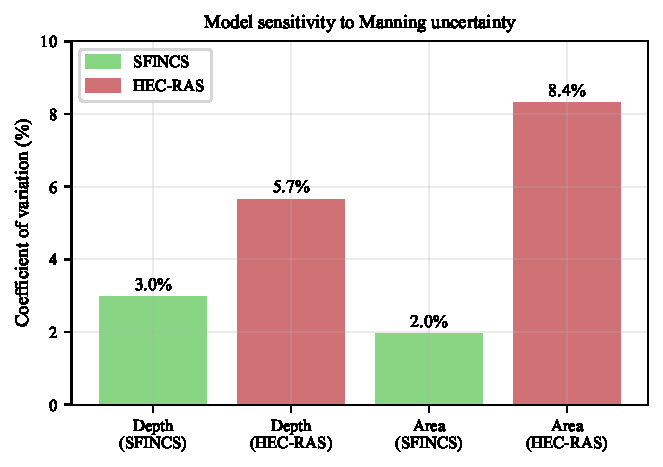
\includegraphics[width=\textwidth]{figures/fig06_cv_comparison.pdf}
%  \caption{Coefficient of variation (CV) of mean water depth and flooded area
%    for \sfincs{} (green) and \hecras{} (red) across 995 Monte Carlo
%    simulations.
%    \hecras{} is $1.9\times$ more sensitive than \sfincs{} for depth
%    (CV: 5.7\% vs.\ 3.0\%) and $4.2\times$ more sensitive for area
%    (CV: 8.4\% vs.\ 2.0\%).
%    Values above bars show the CV to one decimal place.}
%  \label{fig:cv}
%\end{figure}




%% ===========================================================================
\section*{Supplementary Material}
\setcounter{figure}{0}
\setcounter{table}{0}
\renewcommand{\thefigure}{S\arabic{figure}}
\renewcommand{\thetable}{S\arabic{table}}
\renewcommand{\theHfigure}{S\arabic{figure}}
\renewcommand{\theHtable}{S\arabic{table}}

\paragraph{Robustness of main conclusions to inter-class Manning correlation.}
The following figures and table document the Gaussian copula importance-sampling
procedure and its results in full, supporting the correlated-roughness robustness
analysis reported in Section~\ref{sec:res_robustness}.

\begin{figure}[!ht]
  \centering
  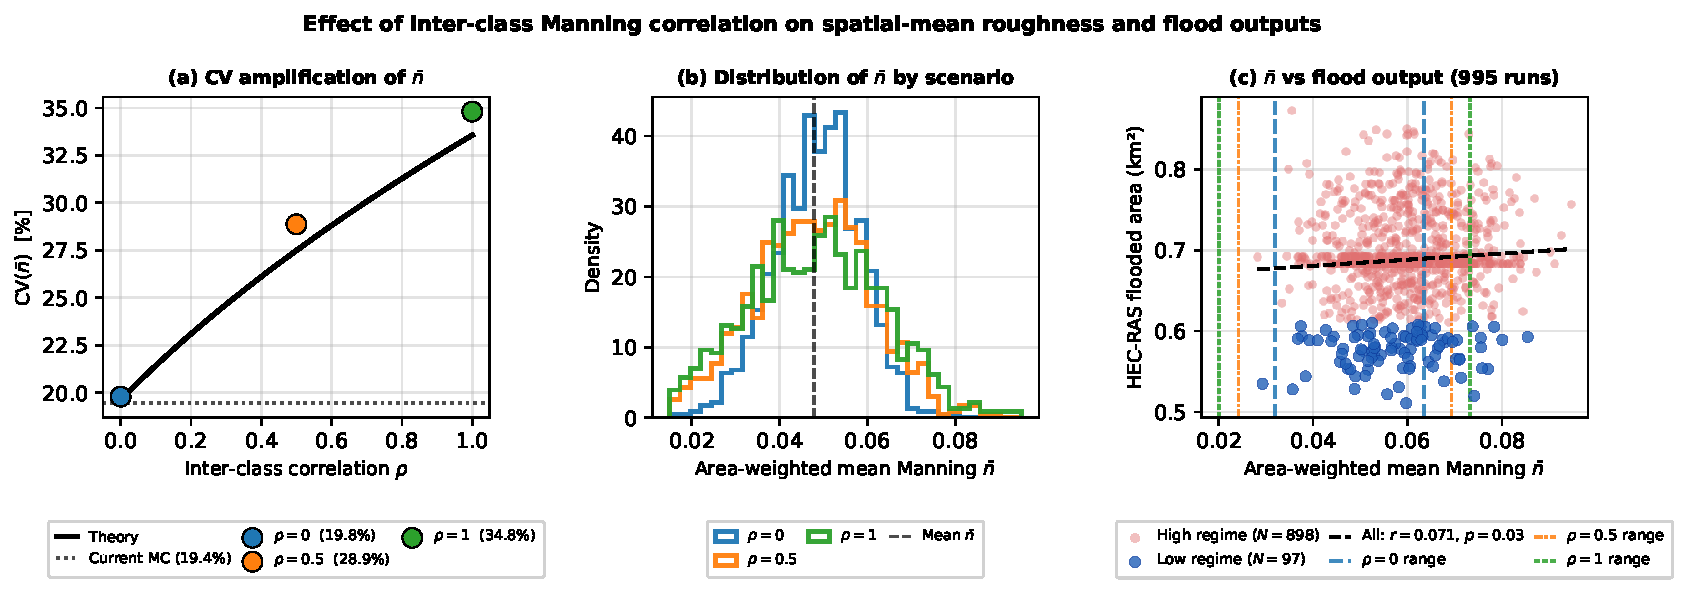
\includegraphics[width=\textwidth]{figures/fig_copula_analysis.pdf}
  \caption{Effect of inter-class Manning correlation on spatial-mean roughness
    and flood outputs ($N = 1\,000$ Gaussian copula samples per scenario).
    (a)~Theoretical CV amplification of the area-weighted mean Manning
    $\bar{n}$ with equi-correlation $\rho$ (solid curve); markers show
    empirical values; dotted line marks the reference independent-MC ensemble.
    (b)~Step histograms of $\bar{n}$: the distribution widens from
    CV\,=\,19.8\% ($\rho=0$) to 34.8\% ($\rho=1$) with no shift in the mean
    ($\bar{n}\approx 0.048$~m$^{-1/3}$s).
    (c)~$\bar{n}$ against HEC-RAS flooded area for 995 valid simulations
    coloured by hydraulic regime (upper-left legend: 5th--95th percentile
    range of $\bar{n}$ per scenario; lower-right legend: regime counts and
    regression); $r=0.071$ ($p=0.03$, $r^2<0.01$) shows only a weak direct
    association between inter-class Manning correlation and domain-scale
    flooded area; the regime fractions under correlated sampling are
    quantified in Supplementary Figure~S3.}
  \label{fig:copula}
\end{figure}

\begin{figure}[!ht]
  \centering
  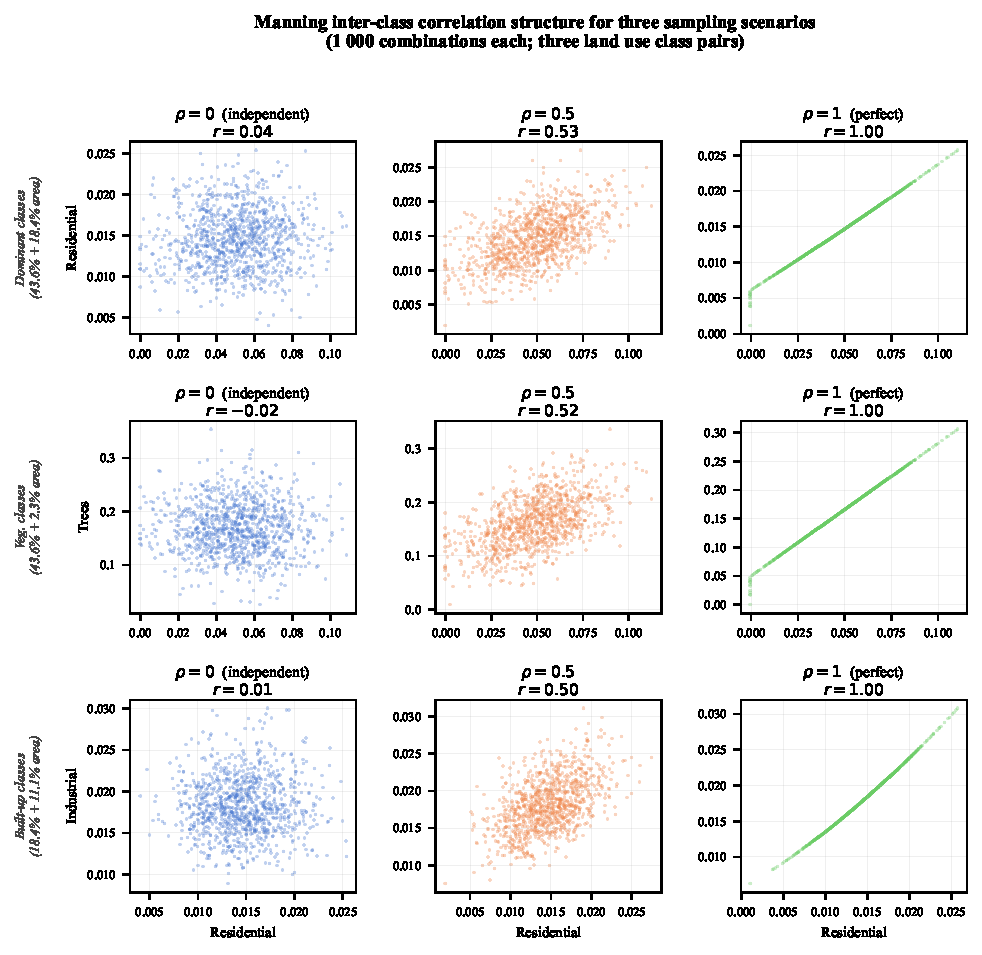
\includegraphics[width=\textwidth]{figures/fig_copula_scatter.pdf}
  \caption{Pairwise scatter plots of Manning $n$ values for three representative
    land use class pairs and three correlation scenarios
    ($N = 1\,000$ Gaussian copula samples each).
    Rows correspond to class pairs (dominant: sparse vegetation + residential;
    vegetation: sparse vegetation + trees; built-up: residential + industrial);
    columns correspond to equi-correlation values
    $\rho \in \{0,\,0.5,\,1.0\}$.
    Empirical Pearson $r$ confirms the copula reproduces the prescribed
    dependence structure.}
  \label{fig:copula_scatter}
\end{figure}

\begin{figure}[!ht]
  \centering
  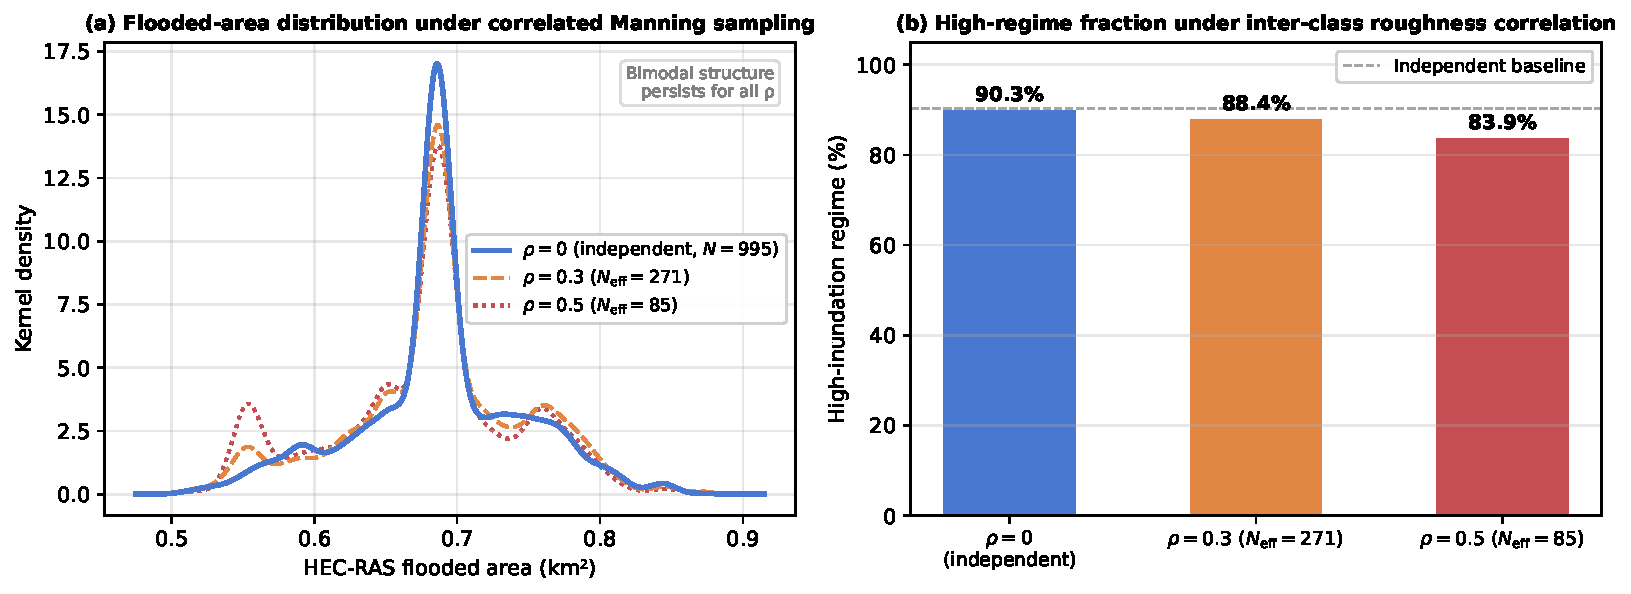
\includegraphics[width=\textwidth]{figures/fig_copula_is.pdf}
  \caption{Importance-sampling robustness check for inter-class Manning correlation.
    (\textbf{a})~Weighted kernel density estimates of \hecras{} flooded area
    under independent sampling ($\rho = 0$, $N = 995$) and two correlated
    scenarios ($\rho = 0.3$, effective $N = 271$; $\rho = 0.5$, effective $N = 85$).
    Weights are the ratio of the equicorrelation Gaussian copula density to
    the independent sampling density, computed from empirical probability
    integral transforms of the 9-class Manning vector.
    The bimodal structure of the \hecras{} response is preserved for all
    values of~$\rho$ shown.
    (\textbf{b})~High-inundation-regime fraction (weighted percentage) as a
    function of equicorrelation~$\rho$.
    The fraction decreases from 90.3\% (independent) to 88.4\% ($\rho = 0.3$)
    and 83.9\% ($\rho = 0.5$), confirming that the bimodal response is robust
    to plausible levels of inter-class roughness correlation.}
  \label{fig:copula_is}
\end{figure}

\begin{figure}[!ht]
  \centering
  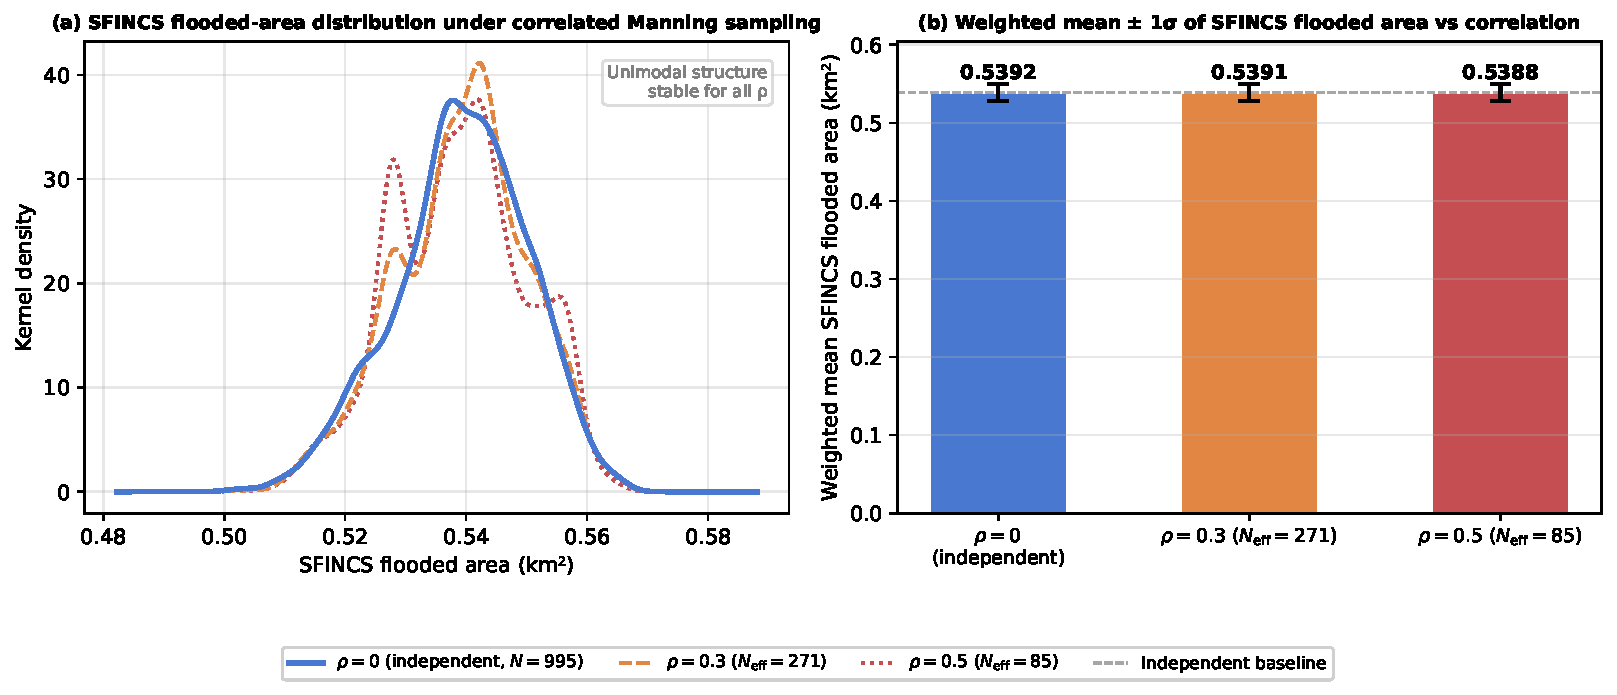
\includegraphics[width=\textwidth]{figures/fig_copula_is_sfincs.pdf}
  \caption{Importance-sampling robustness check for \sfincs{} under inter-class
    Manning correlation (counterpart to Supplementary Figure~S3 for \hecras{}).
    (\textbf{a})~Weighted kernel density estimates of \sfincs{} flooded area
    under independent sampling ($\rho = 0$, $N = 995$) and two correlated
    scenarios ($\rho = 0.3$, effective $N = 271$; $\rho = 0.5$, effective $N = 85$).
    The unimodal distribution is virtually unchanged across all values of~$\rho$.
    (\textbf{b})~Weighted mean $\pm1\sigma$ of \sfincs{} flooded area as a
    function of equicorrelation~$\rho$.
    The mean shifts by less than 0.1\% between $\rho = 0$ (0.5392~km$^2$) and
    $\rho = 0.5$ (0.5388~km$^2$), confirming that the unimodal \sfincs{}
    response is robust to plausible levels of inter-class roughness correlation.}
  \label{fig:copula_is_sfincs}
\end{figure}

\clearpage
\begin{table}[htbp]
  \centering
  \caption{Area-weighted spatial mean Manning $\bar{n}$ statistics under
    independent and Gaussian-copula correlated sampling
    ($N = 1\,000$ draws per scenario; domain area 1\,086~ha).
    P$_5$ and P$_{95}$ denote the 5th and 95th percentiles.}
  \label{tab:copula}
  \begin{tabular}{lcccccc}
    \hline
    Scenario & $\rho$ & Mean $\bar{n}$ & CV(\%) & P$_5$ & P$_{95}$ & P$_{95}$/P$_5$ \\
    \hline
    Independent (reference) & 0   & 0.0484 & 19.4 & 0.033 & 0.064 & 1.94 \\
    Copula $\rho = 0$        & 0   & 0.0486 & 19.8 & 0.032 & 0.063 & 1.98 \\
    Copula $\rho = 0.5$      & 0.5 & 0.0474 & 28.9 & 0.024 & 0.069 & 2.87 \\
    Copula $\rho = 1.0$      & 1.0 & 0.0474 & 34.8 & 0.020 & 0.073 & 3.66 \\
    \hline
  \end{tabular}
\end{table}

\clearpage
\begin{table}[htbp]
  \centering
  \caption{\textbf{Simulations removed prior to analysis} ($N = 5$, 0.5\% of 1\,000).
    Anomalies were detected using a robust $z$-score with threshold
    $k = 5$ (see Section~\ref{sec:metrics_cleaning}).
    Model: S\,=\,SFINCS; H\,=\,HEC-RAS.
    Four of the five anomalies were flagged in HEC-RAS; the SFINCS outputs
    for those four simulations lie within the normal ensemble range.
    Simulation~633 is the exception: the flagged anomaly originates in
    SFINCS (flooded area $= 0.467$~km$^2$), while the paired HEC-RAS
    output falls within the normal ensemble range.
    Ensemble medians for reference: HEC-RAS area $\approx 0.668$~km$^2$,
    depth $\approx 1.22$~m; SFINCS area $\approx 0.537$~km$^2$,
    depth $\approx 1.04$~m.}
  \label{tab:anomalous}
  \resizebox{\textwidth}{!}{%
  \begin{tabular}{cclp{2.4cm}ccccc}
    \toprule
    Sim. & Model & Flagged metric & Flagged value & $|z|_{\mathrm{robust}}$ &
    \multicolumn{2}{c}{HEC-RAS output} & \multicolumn{2}{c}{SFINCS output} \\
    \cmidrule(lr){6-7}\cmidrule(lr){8-9}
    & & & & & Area (km$^2$) & Depth (m) & Area (km$^2$) & Depth (m) \\
    \midrule
    29  & H & Mean depth   & 1.930~m        & 6.70 & 2.187 & 1.930 & 0.498 & 0.949 \\
    295 & H & Mean depth   & 1.772~m        & 5.21 & 1.664 & 1.772 & 0.499 & 0.948 \\
    633 & S & Flooded area & 0.467~km$^{2}$ & 6.84 & 0.865 & 1.545 & 0.467 & 1.005 \\
    724 & H & Mean depth   & 1.805~m        & 5.52 & 1.118 & 1.805 & 0.512 & 0.994 \\
    755 & H & Mean depth   & 1.834~m        & 5.79 & 1.865 & 1.834 & 0.503 & 0.962 \\
    \bottomrule
  \end{tabular}}
\end{table}

\end{document}
